\documentclass[a4paper,11pt,openany]{book}
\usepackage[T1]{fontenc}
\usepackage[utf8]{inputenc}
\usepackage{helvet}
\usepackage{listings}
\usepackage{color}
\usepackage{graphicx}
\usepackage[margin=2cm]{geometry}

\graphicspath{ {Images/} }

\definecolor{codegray}{rgb}{0.5,0.5,0.5}
\definecolor{codegreen}{rgb}{0,0.6,0}
\definecolor{codeblue}{rgb}{0.1,0.1,0.9}
\definecolor{codered}{rgb}{0.9,0.2,0.2}
\definecolor{codebg}{rgb}{0.95,0.95,0.95}

\lstdefinestyle{pystyle}{
  backgroundcolor=\color{codebg},
  commentstyle=\color{codegray},
  keywordstyle=\color{codegreen},
  stringstyle=\color{codered},
  numberstyle=\color{codeblue},
  breaklines=true,
  numbers=left,
  showstringspaces=false,
  showspaces=false,
  showtabs=false,
  tabsize=4,
  basicstyle=\footnotesize
}

\title{Python Tkinter By Example}
\author{David Love}

\newcommand{\myGithub}{http://github.com/Dvlv/tkinter-book}

\begin{document}

\maketitle
\tableofcontents
\newpage

\section{Introduction}
Thank you for taking an interest in my book. Its purpose is to teach you everything you should need to know to begin using Tkinter in Python 3. Examples in this book cover Tkinter 8.6 in Python 3.6. If you wish to follow along using Python 2, there shouldn't be too many differences, but keep in mind I haven't tested the code for compatability. The main thing to note is that the module is likely called \lstinline[columns=fixed]{Tkinter} (capital T), but in Python 3 it is \lstinline[columns=fixed]{tkinter} (small t). 

\vspace{5mm}

Each chapter of this book is written in the form of an image of the target application with the app's entire source code, followed by a breakdown and explanation of the code. Each example is included to teach a specific topic (or a bunch of related ones). Apps are developed iteratively, with each step adding a new feature and teaching a key part. Code which has not changed from the previous iteration will be condensed with ellipses (...) for brevity. I have also included some exercises at the end of each chapter for anyone who wishes to practice development by themselves.

\section{Who this book is aimed at}

This book is written for anyone who knows python and wants to learn a bit about developing GUI applications. Whether you've got a command line application you want to make friendlier with a GUI or you have a great idea for a GUI app which you want to get started on, this book will hopefully give you the tools you need to begin writing your own tkinter apps from scratch.

I will assume that you have basic knowledge of python programming already, and will not explain things like installing python, running programs, or basic syntax (things like \lstinline[columns=fixed]{if}, \lstinline[columns=fixed]{for} loops and such). At the same time, you will not need to be an expert to follow along either. I would suggest learning about \lstinline[columns=fixed]{Class}es if you aren't already aware of them, as all of the examples are written using a class.

\vspace{5mm}

I hope you are able to learn something interesting from this book. Should you have any questions, feel free to contact me. I'm @Dvlv292 on Twitter and Dvlv on Reddit. 

\vspace{5mm}

All source code from this book is freely available on my Github at \myGithub{}.  

\section{How to get the most out of this book}

The best way to ensure that the knowledge from any programming book really sticks in your mind is to \textit{write out the code} for yourself. You can do this whilst reading the section or after finishing the explanation; it doesn't really matter. The important thing is that you code along with the book. Reading the code can only get you so far - you need to practise, practise, practise! 

\vspace{5mm}

Don't just follow along either. If you wonder \textit{"what if I change this"} or \textit{"couldn't I do it like that?"} then just do it! If you mess up, just start again, or grab the code from Github and "reset" back to where you were. You cannot go wrong. 

\section{About tkinter}

\subsection{Installing}

Tkinter is probably already installed alongside python. Some Linux distros may not include it, so you might have to look for \lstinline[columns=fixed]{python3-tkinter} in your package manager. Check by running python in a terminal and trying to do \lstinline[columns=fixed]{>>> import tkinter}. 

\subsection{What is it anyway?}

Tkinter is a GUI library. It comes with everything you would need to begin making GUI applications such as buttons, text inputs, radio buttons, dropdowns, and more. Thanks to its inbuilt module ttk it also has the ability to provide some advanced features like tabbed windows, tree views, and progress bars. 

\subsection{Why write about tkinter?}

I have an unexplainable attachment to tkinter. I think it was the second python module which I began using for a big project - after pygame - and so I just have some nostalgia towards it. Personal preference aside, since tkinter is built into python as part of the standard library, it's pretty much a go-to for new users who want to try out making a GUI. There are no awkward dependencies, no licence issues, and in my opinion it's very easy to pick up and play with. There are lots of great StackOverflow answers for common problems one may run into and the documentation isn't bad either. I think tkinter is the easiest and best library for those who are new to GUI development. Overall though, I'm writing about tkinter because I like it, and I'm having fun writing the apps I'm developing specifically for this book.  

\subsection{I heard tkinter is ugly}

It's true that plain tkinter is not going to win any beauty awards. It's old. The great thing is, tkinter now comes with a module called "ttk" which provides widgets which look native on Windows and OSX (tkinter itself looks very close to native on Linux already). Whilst this book doesn't cover ttk until the last project, after reading it you should be able to swap out the majority of widgets from earlier chapters to ttk's very easily. If you're following along on Windows or OSX don't be put off by the dated styling of tkinter's widgets; once you learn about using and styling ttk widgets in Chapter 7 you should grasp how to make tkinter look great on all platforms.   

\chapter{Hello World}

\section{Basic Example}
As is tradition with all programming books, we'll start with the classic Hello World example to introduce a few things. This will pop up a small window with "Hello World" written inside.

\lstset{style=pystyle}
\lstinputlisting[language=Python, caption=Hello World, captionpos=b]{Code/Chapter1-1.py}

We start with \lstinline[columns=fixed]{root=tk.Tk()} which creates the overall tk window.
Then we define a \lstinline[columns=fixed]{tk.Label()} which will hold our "Hello World" text. The first argument to a Tk widget is the parent in which it will be placed. In this case, we will just put it directly within the \lstinline[columns=fixed]{root} instance.
The \lstinline[columns=fixed]{padx} and \lstinline[columns=fixed]{pady} arguments add padding horizontally and vertically.
\lstinline[columns=fixed]{label.pack()} is then called as a way of placing the label into the root. Other ways of placing widgets, such as \lstinline[columns=fixed]{grid()}, will be covered later.
Finally \lstinline[columns=fixed]{root.mainloop()} is responsible for showing the window.

\vspace{5mm}

Save and run this code and you should see a small window appear with "Hello World" inside, as show here:
\begin{figure}[h]
\centering
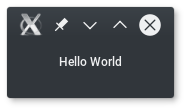
\includegraphics{Ch1-1}
\caption{Our first Tk window}
\end{figure}

\newpage
\section{Using Classes}
Whilst Tkinter code can be written using only functions, it's much better to use a class to keep track of all individual widgets which may need to reference each other. Without doing this, you need to rely on \lstinline[columns=fixed]{global} or \lstinline[columns=fixed]{nonlocal} variables, which gets ugly as your app grows. It also allows for much finer controls once your app gets more complex, allowing you to override default behaviours of Tkinter's own objects.

\lstinputlisting[language=Python, caption=Hello World as a Class, captionpos=b]{Code/Chapter1-2.py}

The main code here is the same as above. The rest is simply creating a \lstinline[columns=fixed]{Root} class inheriting from Tkinter's \lstinline[columns=fixed]{Tk} and running its \lstinline[columns=fixed]{mainloop} function as before. I've also included the standard \break 
\lstinline[columns=fixed]{if "__name__" == __main__} line for familiarity.

\vspace{5mm}

The label now belongs to the Root, rather than being an independent variable. This allows us to reference it easily within methods of the Root class, such as an action we may bind to a \lstinline[columns=fixed]{Button}, which could otherwise be out of scope if we were not using a class.

\vspace{5mm}

Running this code should produce the same small window as in the first example.

\vspace{5mm}

Now we've covered the very basics of making a window appear, let's dive in to something which can actually be used.

\chapter{A To-Do List}
In this chapter we'll be creating a basic to-do list. Here we'll learn about the following:

\begin{itemize}
  \item Allowing the user to enter text
  \item Binding functions to keypresses
  \item Dynamically generating widgets 
  \item Scrolling an area
  \item Storing data (with sqlite)
\end{itemize} 

\section{A Basic List App}

Your first app should look something like this:

\begin{figure}[h]
\centering
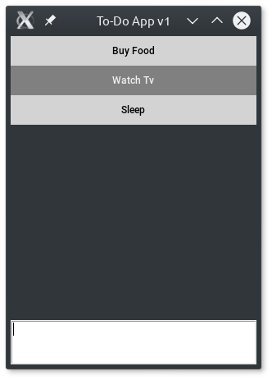
\includegraphics{Ch2-1}
\caption{Our first To-Do App}
\end{figure}

\newpage

Let's get right into the code for the first iteration.

\lstinputlisting[language=Python, caption=Our Initial To-Do Framework, captionpos=b]{Code/Chapter2-1.py}

\subsection{\_\_init\_\_}

We start off by defining our \lstinline[columns=fixed]{Todo} class and initialising it with an empty list of tasks. If using a mutable data-type, such as a list, always ensure you set the default argument to \lstinline[columns=fixed]{None} and convert it into a list within the \lstinline[columns=fixed]{__init__} method, as unexpected behaviour can occur if you try and pass an empty list in. The reasons why are beyond the scope of this book, but you can find great explanations and examples online.

\vspace{5mm}

Next off, we set the title and size of the window. The app can be resized after creation if the user desires, so don't worry too much about getting the initial size perfect. The main reason for this is to signal to the user that the app should be vertically-oriented and prefers to be taller rather than wider. 

\vspace{5mm}

A default task is added to our list to prevent it from just being a big blank space with a text box at the bottom, and to hint to the user what will happen when a task is added. We do this by creating a \lstinline[columns=fixed]{Label}, adding it to our \lstinline[columns=fixed]{tasks} list and packing it. The reason we use a loop to pack this item will become clear when we introduce persistent storage in a later section of this chapter. The \lstinline[columns=fixed]{fg} (foreground) and \lstinline[columns=fixed]{bg} (background) colours are set, and some vertical padding is added for aesthetics. The widgets are packed to the \lstinline[columns=fixed]{TOP} of the window, and are set to fill in the \lstinline[columns=fixed]{X} direction, i.e. horizontally, to ensure they are all of uniform width, and the background spans the entirety of the window. 

\vspace{5mm}

The final widget we need is our \lstinline[columns=fixed]{Text} box, which is what the user will type into. We shorten the default \lstinline[columns=fixed]{height} to 3 to make it look a bit nicer, and specify the white background with black text to look more like traditional text inputs. After packing it at the \lstinline[columns=fixed]{BOTTOM} of our window spanning the full \lstinline[columns=fixed]{X} direction like our tasks, we call \lstinline[columns=fixed]{focus_set} so that the cursor is inside the box when the window is opened. Without this, the user would have to click inside the box before they could type anything. We then bind the \lstinline[columns=fixed]{Return} (or Enter) key to a function \lstinline[columns=fixed]{add_item} which we will get to next. A note when binding - do not put the parentheses at the end of the function name. We want to pass the function itself across, but if we put the parentheses we will end up calling the function instead. 

\vspace{5mm}

The last thing to do is define our colour schemes. This is used to better separate individual items from the list view. I've gone for light grey with black text, followed by darker grey with white text. Feel free to switch these up to suit your preferences. You may notice the default list item has the styling of the first scheme, so as to ensure it fits the pattern. The \lstinline[columns=fixed]{colour_schemes} variable is a list of dictionaries containing a background and foreground colour, which we will use to alternate the styles when adding new tasks.  

\subsection{add\_item}

When adding a new item, the first thing to do is get the text which the user entered into our \lstinline[columns=fixed]{Text} widget. The arguments here tell the widget how much of the text to grab. \lstinline[columns=fixed]{1.0} tells it to begin at the first character, and the \lstinline[columns=fixed]{END} constant tells it to look until the end of the box. We also call \lstinline[columns=fixed]{strip()} on the result to remove the newline character which is entered when the user presses \lstinline[columns=fixed]{Return} to submit the text, as well as any trailing space characters. 

\vspace{5mm}

We need to check if the length of the entered text is greater than \lstinline[columns=fixed]{0} to avoid letting the user add blank tasks. If this is true, then we create a new \lstinline[columns=fixed]{Label} with the text entered by the user. The \lstinline[columns=fixed]{divmod} function is used to determine whether we are on an even or odd number of total tasks, allowing us to set the correct styling to our new label. \lstinline[columns=fixed]{Divmod} returns the quotient and remainder when the first argument is divided by the second. In our case, we want the remainder when the size of our list is divided by 2. The quotient is set to \lstinline[columns=fixed]{_}, which is commonly used in python to denote a variable which we do not plan on using. The remainder is then used as the index of our \lstinline[columns=fixed]{colour_schemes} list to grab the correct foreground and background colour dictionary. The \lstinline[columns=fixed]{configure} method is used to set a property of a widget, just as you would pass the values in as keyword arguments when creating them initially. We set the foreground and background colours of our \lstinline[columns=fixed]{Label} with the chosen dictionary's values, and then pack it the same way as our default item. Finally, we add this to the \lstinline[columns=fixed]{tasks} variable so as to keep count of how many items we have.

\vspace{5mm}

We clear everything written in the \lstinline[columns=fixed]{Text} widget outside of our \lstinline[columns=fixed]{if} statement. This is to prevent the user from adding newlines before their task name by pressing \lstinline[columns=fixed]{Return} before typing anything. We also want to clear it if they have entered a task, so they do not have to delete it manually before writing another. 

\subsection{Next Iteration}

That's it for the first iteration of our to-do list! We now have a styled list of items which can be added to. Whilst playing with this example, you will probably notice that if you add too many items, you need to re-size the window to see any more. You also cannot delete any items which you may have completed. These will both be addressed next. 

\newpage

\section{Scrolling and Deleting}

A lot has changed from the previous iteration, so I will include the full code in this section. Your new To-do app can be written as follows:

\lstinputlisting[language=Python, caption=Our Scrolling To-Do, captionpos=b]{Code/Chapter2-2.py}

\newpage

\subsection{Canvases and Frames}

With this re-write, I have introduced some new components - a \lstinline[columns=fixed]{Canvas} and two \lstinline[columns=fixed]{Frames}. A \lstinline[columns=fixed]{Canvas} is a powerful general-use widget with many capabilities (usually graphical). We are using it here for its ability to scroll, which we need if we want to add a lot of apps to our list. A \lstinline[columns=fixed]{Frame} is a layout component which can be used to group together multiple other widgets. As you will see in this case, we can actually use the \lstinline[columns=fixed]{Canvas} to draw a \lstinline[columns=fixed]{Frame} into our window, which is then able to bundle together all of our to-do items, allowing them to scroll independently of the \lstinline[columns=fixed]{Text} widget we use to add new tasks.

\subsection{\_\_init\_\_}

As above, we now create a \lstinline[columns=fixed]{Canvas} and two \lstinline[columns=fixed]{Frames}, with one \lstinline[columns=fixed]{Frame} parented to the canvas, and the other to the main window. We then make a \lstinline[columns=fixed]{Scrollbar} object to allow scrolling of the page. We set the orientation and command to tell tkinter that we want a vertical scrollbar, scrolling in the y direction. We also configure our canvas to accept the \lstinline[columns=fixed]{Scrollbar}'s values. We once again set the window title and size, and create our \lstinline[columns=fixed]{Text} widget - this time parented to one of the frames (which will be packed to the bottom). Our \lstinline[columns=fixed]{Canvas} is packed with instruction to fill all available space and expand as big as it can, and our \lstinline[columns=fixed]{Scrollbar} follows, filling up the vertical space. 

\vspace{5mm}

The next line looks a little strange. We use our \lstinline[columns=fixed]{Canvas} to create a new window inside itself, which is our \lstinline[columns=fixed]{Frame} holding the tasks. We create it at the coordinates \lstinline[columns=fixed]{(0,0)} and anchor it to the top of the \lstinline[columns=fixed]{Canvas} (the "n" here is for "north", so top-left would require "nw", and so on). One thing to note is that we do \textbf{not} pack our \lstinline[columns=fixed]{tasks_frame}, as it will not appear, and we will be left scratching our heads as to where it is. This is something I learned the hard way!

\vspace{5mm}

After that, we \lstinline[columns=fixed]{}\lstinline[columns=fixed]{pack} our \lstinline[columns=fixed]{Text} into its frame and then \lstinline[columns=fixed]{}\lstinline[columns=fixed]{pack} its frame to the \lstinline[columns=fixed]{BOTTOM} of the window, with both filling the \lstinline[columns=fixed]{X} direction. The default task is created and we bind the \lstinline[columns=fixed]{self.remove_task} function to it being clicked (this will be covered below). We pack this, and then move on to a big block of binds. The \lstinline[columns=fixed]{<MouseWheel>}, \lstinline[columns=fixed]{<Button-4>} and \lstinline[columns=fixed]{<Button-5>} binds handle scrolling, and the \lstinline[columns=fixed]{<Configure>} binds handle keeping the \lstinline[columns=fixed]{Canvas} as big as possible as the window changes size. The \lstinline[columns=fixed]{<Configure>} event is fired when widgets change size (and on some platorms, location) and will provide the new width and height. The \lstinline[columns=fixed]{<Return>} bind and \lstinline[columns=fixed]{colour_schemes} remain from the previous example. 

\subsection{Handling Tasks}

The \lstinline[columns=fixed]{add_task} method is almost the same as the previous iteration, but the code for choosing the styling has been moved into a separate method - \lstinline[columns=fixed]{set_task_colour} - so that it can be re-used after deleting tasks. Speaking of which, we have a \lstinline[columns=fixed]{remove_task} method which will handle getting rid of the \lstinline[columns=fixed]{Label} widget associated with the task. To avoid accidental removal, we use an \lstinline[columns=fixed]{askyesno} pop-up message to double-check with the user that they wanted to delete that task (make sure you don't miss the new \lstinline[columns=fixed]{import tkinter.messagebox as msg} statement at the top of the file). This will create a small notice with the title "Really Delete?" and the message "Delete <task>?" (where <task> will be the text within the \lstinline[columns=fixed]{Label}) with the options "yes" and "no". Using the \lstinline[columns=fixed]{if} statement around this means the indented code will only happen if the user presses "yes". Upon deletion, we recolour all remaining tasks in our alternating pattern, as otherwise the pattern would be broken by the removal.  

\subsection{Adjusting the canvas}

Our \lstinline[columns=fixed]{on_frame_configure} method is bound to our \lstinline[columns=fixed]{root}'s \lstinline[columns=fixed]{<Configure>} action, and will be called whenever the window is resized. It sets the scrollable region for our canvas, and uses the \lstinline[columns=fixed]{bbox} (bounding box) to specify that we want the entire canvas to be scrollable. The \lstinline[columns=fixed]{task_width} method is bound to the \lstinline[columns=fixed]{Canvas}'s \lstinline[columns=fixed]{<Configure>}, and is responsible for ensuring the task \lstinline[columns=fixed]{Label}s stay at the full width of the canvas, even after stretching the window.

\subsection{Mouse scrolling}

Our final method, \lstinline[columns=fixed]{mouse_scroll}, is how we bind scrolling to the mouse wheel as well as the scrollbar. This is bound to \lstinline[columns=fixed]{<MouseWheel>} for Windows and OSX, and to \lstinline[columns=fixed]{<Button-4>} and \lstinline[columns=fixed]{<Button-5>} for Linux. We then simply call the \lstinline[columns=fixed]{Canvas}' \lstinline[columns=fixed]{yview_scroll} method based upon whether we receive a \lstinline[columns=fixed]{delta} or a \lstinline[columns=fixed]{num} within the event. Here on Linux I get a \lstinline[columns=fixed]{num}. The delta is usually 120 or -120, so is divided by 120 for more precise scrolling, and multiplied by -1 to adjust the direction.  

\subsection{Next Iteration}

Our final iteration will handle saving and retrieving values from a \lstinline[columns=fixed]{sqlite} database. I have left this until last because it's not strictly \lstinline[columns=fixed]{tkinter} related, and so you are free to skip this section if you have no interest in learning about databases, or you already know enough to figure out how to do this on your own. If you think the latter is true, please do go ahead and try as an exercise before reading this section. 

\newpage

\section{Permanent Storage}

There are only a few small changes to our existing methods in this iteration, so I will not re-print the whole class. If you wish to follow along, start with your code from the previous version, make the changes listed in this section, and add any other new methods to the end of our \lstinline[columns=fixed]{Todo} class. As a reminder, the full code will be available on Github at \myGithub{} as \lstinline[columns=fixed]{Chapter2-3.py}.

\lstinputlisting[language=Python, caption=Database Integration, captionpos=b]{Code/Chapter2-3-abridged.py}

\newpage

\subsection{runQuery}

Let's start by explaining the database handling. Our \lstinline[columns=fixed]{runQuery} method is a fairy generic database handling method. It takes an sql string, some data to format into the sql string, and \lstinline[columns=fixed]{receive} which indicates to the method whether or not it needs to return any data (from a \lstinline[columns=fixed]{SELECT} statement). We first connect to our database file, in this case \lstinline[columns=fixed]{tasks.db}, and receive a \lstinline[columns=fixed]{cursor}. The \lstinline[columns=fixed]{cursor} is used to execute queries against the database and sometimes return data. We then close off our connection at the end to reduce resource usage. This is a static method so that it can be called by our proceeding \lstinline[columns=fixed]{firstTimeDb} method, which needs to be called before our \lstinline[columns=fixed]{__init__}, and so is also static.

\subsection{firstTimeDb}

This function is used to create the database file, \lstinline[columns=fixed]{tasks.db}, if it does not already exist. We also put our old default task, \lstinline[columns=fixed]{--- Add Tasks Here ---}, in this method so that it appears when the user first loads the app, but is permanently deletable like other tasks. 
 
\subsection{\_\_init\_\_}

We start by just updating the window's title bar to the 3rd version. We move the existing \lstinline[columns=fixed]{colour_schemes} variable to above the new code which will populate our existing tasks, so that we can use it during the initial set-up. Without doing this, we would get an error when we reference it via \lstinline[columns=fixed]{add_task}. Instead of the hard-coded default task, we now fetch existing tasks from the database with \lstinline[columns=fixed]{load_tasks}, then iterate through them, passing each to our slightly altered \lstinline[columns=fixed]{add_task} method.

\subsection{add\_task and remove\_task}

To prevent re-writing most of this code in our \lstinline[columns=fixed]{__init__} method, we have added two new parameters to \lstinline[columns=fixed]{add_task}: \lstinline[columns=fixed]{task_text} and \lstinline[columns=fixed]{from_db}. This allows us to pass in text independent of our \lstinline[columns=fixed]{Text} widget, and to prevent re-saving tasks to the database which originated from there. Before destroying our widget inside \lstinline[columns=fixed]{remove_task}, we grab its text and remove it from the database too. 

\subsection{save\_task and load\_tasks}
These two methods deal with database access. \lstinline[columns=fixed]{save_task} will add a new task into our database, and \lstinline[columns=fixed]{load_tasks} is called in our \lstinline[columns=fixed]{__init__} method to retrieve all saved tasks when loading the app. These two methods ensure that the task list displays the same when the user closes then re-opens the app.

\subsection{The final app}

That's it for our to-do list. We now have a to-do application which can save and retrieve tasks which remain after closing the app. We have learned how to layout multiple widgets with \lstinline[columns=fixed]{Frame}s and the \lstinline[columns=fixed]{pack} method, how to make a scrollable area which maintains its size when the window is resized, how to bind methods to user inputs and \lstinline[columns=fixed]{tkinter}'s own events, and how to dynamically add and remove widgets based on user actions. If you read the final section, you will also know how to integrate \lstinline[columns=fixed]{tkinter} nicely with a \lstinline[columns=fixed]{sqlite} database. Next up we will create an app which utilises a tabbed interface, also known as a \lstinline[columns=fixed]{Notebook}.

\subsection{Further Development}

If you'd like to continue work on this project as an exercise, try the following:

\begin{itemize}
  \item Prevent duplicate tasks by using a database look-up before adding a new task.
  \item Give each task a "Delete" button instead of the on-click event on the Label itself (Buttons will be covered next chapter).
  \item Instead of destroying tasks, mark them as "finished" using a column in the database and display them as "greyed out". 
  \item Add a "category" for each task and colour the task based on the category instead of using the pattern (maybe separate them with a border).
\end{itemize} 

\chapter{A Multi-Language Translation Tool}

In this chapter we'll be creating a tool which will translate english text into multiple other languages using the Google Translate API. Here we'll learn about the following:

\begin{itemize}
  \item Creating a tabbed interface
  \item Creating a Menu
  \item Creating a pop-up window
  \item Accessing the Clipboard 
  \item Calling APIs with \lstinline[columns=fixed]{requests}
\end{itemize} 

\section{A Single-Translation Interface}

We'll start with a simple app which translates to one language (italian). Your first app should look something like this:

\begin{figure}[h]
\centering
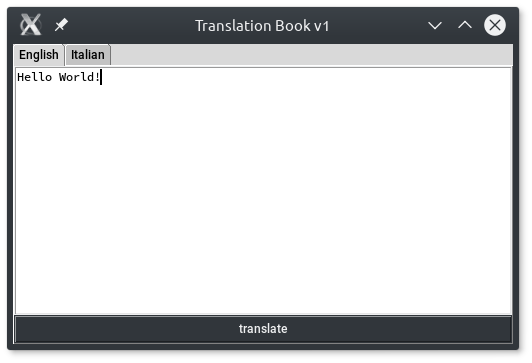
\includegraphics{Ch3-1-1}
\caption{A two-tabbed translator (English)}
\end{figure}

\newpage

\begin{figure}[h]
\centering
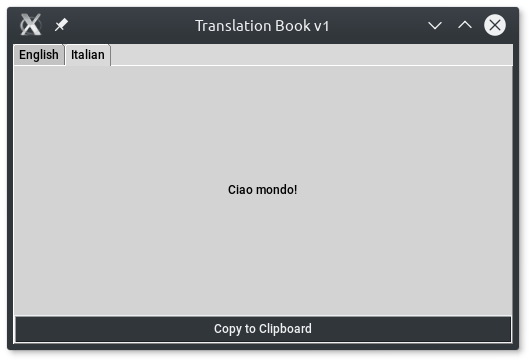
\includegraphics{Ch3-1-2}
\caption{A two-tabbed translator (Italian)}
\end{figure}

\lstinputlisting[language=Python, caption=Our first translation app, captionpos=b]{Code/Chapter3-1.py}

\subsection{requests}

We now import and use the \lstinline[columns=fixed]{requests} module. If you do not have this installed, you can get it with pip (\lstinline[columns=fixed]{pip install requests}).

\subsection{\_\_init\_\_}

Hopefully most the \lstinline[columns=fixed]{__init__} should look familiar to you by now. The first new bit is the creation of a \lstinline[columns=fixed]{Notebook}, which is what holds our tabs. The contents of each notebook tab is simply a \lstinline[columns=fixed]{Frame}, each of which holds two elements. Our \lstinline[columns=fixed]{english_frame} holds a \lstinline[columns=fixed]{Text} widget, allowing the user to enter some text, and a \lstinline[columns=fixed]{Button} which triggers the translation. The \lstinline[columns=fixed]{command} argument supplied to a \lstinline[columns=fixed]{Button} is the function which we want to be called when it is clicked. An important thing to remember is to \textbf{not} put the parentheses at the end of the function name, as this will actually call the function and bind the result (we want to bind the function itself). This is the same potential mistake as when binding with the \lstinline[columns=fixed]{bind} method from chapter 1.

\vspace{5mm}

Our \lstinline[columns=fixed]{italian_frame} holds an expanded \lstinline[columns=fixed]{Label} instead of a \lstinline[columns=fixed]{Text} input, as we don't want to be able to alter the translated text, as well as a \lstinline[columns=fixed]{Button} which will copy the translated text to our computer's clipboard.  

\vspace{5mm}

Another new thing here is the use of a \lstinline[columns=fixed]{StringVar}. As you may be able to guess from the name, this is like a sophisticated container for a string variable, which allows us the change the text of a \lstinline[columns=fixed]{Label} without needing to re-configure it. Its other great use is changing the text of multiple \lstinline[columns=fixed]{Label}s (which need to say the same thing) all at once, and we can also fire callbacks whenever the variable changes. In our case, the \lstinline[columns=fixed]{StringVar} is used to update the \lstinline[columns=fixed]{Label} containing our italian translation, and to grab the text back out to put onto our clipboard (as we'll see later).

\vspace{5mm}

Instead of \lstinline[columns=fixed]{pack}ing our two frames, we just \lstinline[columns=fixed]{add} them to our notebook and pass the \lstinline[columns=fixed]{text} (i.e. the name of the tab) along with them, before finally \lstinline[columns=fixed]{pack}ing our \lstinline[columns=fixed]{Notebook}. Hopefully you should have a good idea of the use-cases of this app just from the \lstinline[columns=fixed]{__init__} method.

\subsection{translate}

Much like with our to-do app, we grab the user's text from our \lstinline[columns=fixed]{Text} widget, but we won't clear it this time in case they've typed something really long and want to add something after translation. We next create the URL to access google translate's API with the \lstinline[columns=fixed]{format} method, passing in our original language code ("en"), target language code (defaults to "it", but we will specify this when adding another tab next iteration) and our text to be translated (which we grabbed from the \lstinline[columns=fixed]{Text} widget earlier). We visit this URL using the \lstinline[columns=fixed]{requests} module's \lstinline[columns=fixed]{get} method. The \lstinline[columns=fixed]{raise_for_status} method will raise an \lstinline[columns=fixed]{Exception} should we recieve an error when calling the API, such as a 404 if there's a typo. For this reason, we've put our code in a \lstinline[columns=fixed]{try / except} block so that we can gracefully alert the user via a \lstinline[columns=fixed]{messagebox} if there's a problem. If no \lstinline[columns=fixed]{Exception}s are raised, we use the \lstinline[columns=fixed]{json} method of \lstinline[columns=fixed]{requests} to parse the json-formatted response from the API into a nice block of python lists. The translation is in the first element of the first element of the first list (not too graceful, I know!), hence the chaining of \lstinline[columns=fixed]{[0][0][0]}. If you wish to look at the response, add a \lstinline[columns=fixed]{print(translation)} on the next line. We finish up by setting the translated text as the value of our \lstinline[columns=fixed]{StringVar} and showing the user a success message so that they know the other tabs have updated.

\subsection{copy\_to\_clipboard}  

This is the function bound to the \lstinline[columns=fixed]{Button} in our italian tab. We simply grab the \lstinline[columns=fixed]{StringVar}'s value (which our \lstinline[columns=fixed]{Label} holds) and use \lstinline[columns=fixed]{tkinter} to add the text into our computer's clipboard. I originally intended to use the \lstinline[columns=fixed]{pyperclip} module to handle the clipboard, but then I found out that \lstinline[columns=fixed]{tkinter} can handle it already - super handy!

\subsection{Next Iteration}

Now that we have a proof-of-concept for our translator, we'll go deeper in and set up a second language for us to translate to, as well as a menu for us to pick languages from. 

\newpage

\section{Three Tabs and a Menu}

\begin{figure}[h]
\centering
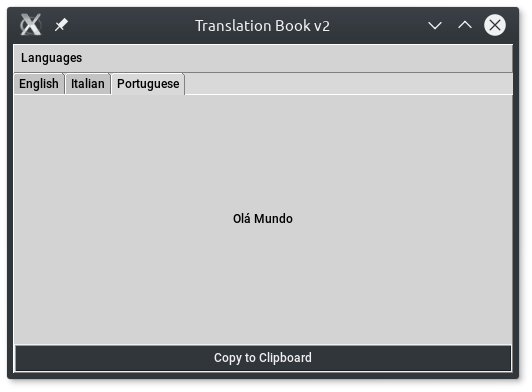
\includegraphics{Ch3-2}
\caption{A portuguese translation in our notebook}
\end{figure}

Our next iteration boasts a menu bar at the top, and the ability to translate to both italian and portuguese at once. After running this iteration, click the "Languages" menu - you should see a "Portuguese" option. Selecting this will add a third tab to our \lstinline[columns=fixed]{Notebook}. If we follow the same translation process as before, we will now see both the italian and portuguese tabs are updated with the translations. Neat. Whilst this is not yet fully dynamic, we've laid out some groundwork for alternative translations. Let's take a look at the code changes which make this possible.

\newpage 

\lstinputlisting[language=Python, caption=Our Translator with a Menu, captionpos=b]{Code/Chapter3-2-abridged.py}

\subsection{\_\_init\_\_}

We now encounter a new \lstinline[columns=fixed]{tkinter} widget - a \lstinline[columns=fixed]{Menu}. A \lstinline[columns=fixed]{Menu} is essentially a container for a list of buttons. We start by declaring our "overall" menu, \lstinline[columns=fixed]{self.menu}, which will hold our submenu, \lstinline[columns=fixed]{self.languages_menu}. We set \lstinline[columns=fixed]{tearoff} to 0 so that the user can't drag-and-drop the languages submenu out of the main menu. We then add a command (essentially a button) called Portuguese. We bind the \lstinline[columns=fixed]{add_portuguese_tab} method to this button, again making sure not to call the function. We then use \lstinline[columns=fixed]{add_cascade} to place our submenu into our main bar. We finish up by calling \lstinline[columns=fixed]{self.configure(menu=self.menu)} to set the root window's menu to our overall menu.  

\vspace{5mm}
 
The only other change to this method is the moving of the \lstinline[columns=fixed]{italian_translation StringVar} to above our \lstinline[columns=fixed]{translate_button} so that we can use it in the \lstinline[columns=fixed]{command}. Speaking of which, we've now changed this to a \lstinline[columns=fixed]{lambda} which calls the new-and-improved translate method with a couple of lists as arguments. Let's look into \lstinline[columns=fixed]{translate} now.


\subsection{translate}

Our \lstinline[columns=fixed]{translate} now takes another argument - \lstinline[columns=fixed]{elements} - which is a list of \lstinline[columns=fixed]{StringVar}s to update with a translation. The \lstinline[columns=fixed]{target_languages} argument is now expected to be a list of language codes, and the name has been pluralised to reflect this. 

\vspace{5mm}

Our \lstinline[columns=fixed]{url} is no longer formatted upon creation, but is instead left with the placeholders in. We use \lstinline[columns=fixed]{zip} to combine our lists of language codes and \lstinline[columns=fixed]{StringVar} elements into the correct pairs and then use them to format our URL, parse out the translation, and update the \lstinline[columns=fixed]{StringVar} as before - but this time in a loop, allowing us to do this for any number of languages. You may not have come across an \lstinline[columns=fixed]{else} by a \lstinline[columns=fixed]{try / except} block before. The purpose of the \lstinline[columns=fixed]{else} is to execute code only if there was no exception caught in the \lstinline[columns=fixed]{except}. We've put our success \lstinline[columns=fixed]{messagebox} in this \lstinline[columns=fixed]{else} because we only want it to show once, so it couldn't be left inside the \lstinline[columns=fixed]{for} loop, and we don't want it to show if, say, the first translation worked but the second did not. Out there in the \lstinline[columns=fixed]{else} it should not be able to mislead the user into thinking the translation was successful if it wasn't, and will only appear once at the end of the process.

\subsection{add\_portuguese\_tab}

This is the function called when we choose our "Portuguese" option from our "Languages" menu. A lot of the code here looks just like the italian code from our \lstinline[columns=fixed]{__init__}. Since our \lstinline[columns=fixed]{copy_to_clipboard} method still has all of the defaults set to the italian translations, our \lstinline[columns=fixed]{portuguese_copy_button} instead uses a lambda to call it with the \lstinline[columns=fixed]{text} argument as the value of its \lstinline[columns=fixed]{portuguese_translation StringVar}. 

\vspace{5mm}

At the end of the function we disable the "Portuguese" entry in our "Languages" menu. Without this we could create multiple Portuguese tabs, which is pointless. We finish off by changing the \lstinline[columns=fixed]{command} of our translate button to a new \lstinline[columns=fixed]{lambda} which contains both the italian and portuguese language codes and \lstinline[columns=fixed]{StringVar}s.   

\subsection{Next Iteration}

You may notice this code feels a bit hacky. The \lstinline[columns=fixed]{add_portuguese_tab} function knows (well, assumes) that we have an italian tab, and directly modifies our translate button too. In order to generalise this for re-use we're going to look at making each translation \lstinline[columns=fixed]{Frame} its own class - allowing us to make any language supported by google translate and add it as a tab to our notebook. The reason we didn't do this all in one go was so that we could meet the \lstinline[columns=fixed]{Menu} widget and lay the groundwork for dynamically adding tabs before a big overhaul of the app.

\newpage

\section{A Truly Dynamic App}

Our code is now split into 3 classes which I will cover separately. The executable code for this section is all in Chapter3-3.py for those downloading it from Github. It is best practice to keep to one class per file, but for the sake of book simplicity I've combined them. We'll start this section off by looking at the new \lstinline[columns=fixed]{LanguageTab} class. 

\subsection{The LanguageTab}

\lstinputlisting[language=Python, caption=An Independent Language Tab, captionpos=b]{Code/Chapter3-3-LanguageTab.py}

Our \lstinline[columns=fixed]{LanguageTab} class is built on top of a \lstinline[columns=fixed]{Frame}, since that's what we \lstinline[columns=fixed]{add} into our \lstinline[columns=fixed]{Notebook}. It holds a reference to the full name of the language (for the tab name) and its short code for the google translate API. It is responsible for its own \lstinline[columns=fixed]{StringVar}, \lstinline[columns=fixed]{Label} and \lstinline[columns=fixed]{Button}, as well as the command bound to the \lstinline[columns=fixed]{Button}

\vspace{5mm}

The \lstinline[columns=fixed]{copy_to_clipboard} method needs to access the root window, i.e. our \lstinline[columns=fixed]{TranslateBook} instance, because that's what has control over the clipboard. We grab this with the \lstinline[columns=fixed]{winfo_toplevel} method, then use the same code as before to put our \lstinline[columns=fixed]{StringVar}'s contents onto the clipboard.

\vspace{5mm}

Now we'll jump back to the main \lstinline[columns=fixed]{TranslateBook} class which handles our root window.

\newpage

\subsection{The TranslateBook}

\lstinputlisting[language=Python, caption=Our Main Class, captionpos=b]{Code/Chapter3-3-TranslateBook.py} 

\subsubsection{\_\_init\_\_}

We've added a new item to our \lstinline[columns=fixed]{languages_menu} - add new - which will be covered with our final class \lstinline[columns=fixed]{NewLanguageForm}. We've also re-written our portuguese entry to use a new method \lstinline[columns=fixed]{add_new_tab}. We no longer make everything for our italian tab since this is handled with the \lstinline[columns=fixed]{LanguageTab} class, we instead keep a list of tabs inside \lstinline[columns=fixed]{self.language_tabs}. Since our english tab is different, we still have all of the set up of that here.

\subsubsection{translate}

This should still look very familiar. Instead of passing in a list of language codes and elements, we just grab our list of \lstinline[columns=fixed]{language_tab}s and pull the codes and elements from each instance. If we have no language tabs a \lstinline[columns=fixed]{messagebox} will alert the user to add one first and exit the method with \lstinline[columns=fixed]{return}. 

\subsubsection{add\_new\_tab} 

We pass this method a \lstinline[columns=fixed]{LanguageTab} object and it gets appended to our \lstinline[columns=fixed]{language_tabs} list and added to our \lstinline[columns=fixed]{Notebook}. We also try to disable the \lstinline[columns=fixed]{menu} entry if it exists. We don't mind if this fails, as it likely means the language was created outside of the menu and there's no entry to disable, so we can just \lstinline[columns=fixed]{pass} if an \lstinline[columns=fixed]{Exception} is thrown. 

\subsubsection{show\_new\_language\_popup}

All we need to do here is create the \lstinline[columns=fixed]{NewLanguageForm} instance which will handle everything else. Let's look at this now.

\newpage

\subsection{NewLanguageForm}

\begin{figure}[h]
\centering
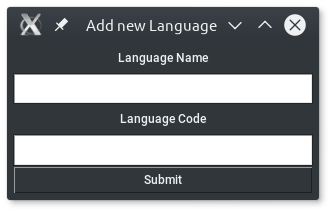
\includegraphics{Ch3-3}
\caption{Our Add New Language Form}
\end{figure}

\lstinputlisting[language=Python, caption=Our Translator with a Menu, captionpos=b]{Code/Chapter3-3-NewLanguageForm.py}
 
As you should be able to interpret from the code, we have a small window with 2 \lstinline[columns=fixed]{Label}s, 2 \lstinline[columns=fixed]{Entries} and a \lstinline[columns=fixed]{Button}. An \lstinline[columns=fixed]{Entry} is just a \lstinline[columns=fixed]{Text} widget which is only one line. If you're familiar with HTML, think of an \lstinline[columns=fixed]{Entry} as an \lstinline[columns=fixed]{input[type="text"]} and a \lstinline[columns=fixed]{Text} as a \lstinline[columns=fixed]{textarea}. Our \lstinline[columns=fixed]{__init__} just sets our window title and size, creates the widgets, and packs them all. The \lstinline[columns=fixed]{master} argument to here is our \lstinline[columns=fixed]{TranslateBook} instance, as the \lstinline[columns=fixed]{submit} method needs to access its \lstinline[columns=fixed]{languages_menu}

\vspace{5mm}

Our \lstinline[columns=fixed]{submit} method is called by our \lstinline[columns=fixed]{Button}. It grabs the text from our two \lstinline[columns=fixed]{Entries} and creates a \lstinline[columns=fixed]{LanguageTab} instance from them. It then accesses our \lstinline[columns=fixed]{TranslateBook}'s \lstinline[columns=fixed]{languages_menu} and adds the newly created \lstinline[columns=fixed]{LanguageTab} instance as an option. Finally it shows a success \lstinline[columns=fixed]{messagebox} and destroys itself (so the user doesn't have to close it manually). If you don't like this, you could always clear the \lstinline[columns=fixed]{Entries} and leave the window open for the user to add another language straight after. If the user hasn't filled out one of the \lstinline[columns=fixed]{Entries} a \lstinline[columns=fixed]{messagebox} will let them know that they are both needed. 

\subsection{Running this version}

In our old \lstinline[columns=fixed]{if __name__ == "__main__"} statement we just created a \lstinline[columns=fixed]{TranslateBook} instance and called its \lstinline[columns=fixed]{mainloop}. If we want tabs to appear by default, like our italian tab originally, we need to create a \lstinline[columns=fixed]{LanguageTab} instance and then use \lstinline[columns=fixed]{add_new_tab} to add it to our \lstinline[columns=fixed]{TranslateBook} before calling \lstinline[columns=fixed]{mainloop}. In Chapter3-3.py you will see I have done this with the italian tab as before. 

\vspace{5mm}

If you don't know of a language and code to test the \lstinline[columns=fixed]{NewLanguageForm} out with, try "Spanish" and "es". Keep in mind that we only add the new language as a menu option, so it will not appear in your \lstinline[columns=fixed]{Notebook} straight away, you must pick it from the menu first. 

\subsection{Further Development}

If you'd like to continue work on this project as an exercise, try the following:

\begin{itemize}
  \item Import \lstinline[columns=fixed]{ttk} and adjust the app to use \lstinline[columns=fixed]{ttk}'s widgets (you will see a small attempt at this with Chapter3-3-ttk.py on Github, as I eventually deemed it unworthy of its own section).
  \item Bind the relevant \lstinline[columns=fixed]{Button} functionality to the \lstinline[columns=fixed]{Return} key.
  \item Before adding a new language validate that the short code added exists for the google translate api.
  \item Remember the app's previous state with \lstinline[columns=fixed]{sqlite} (i.e. which tabs were added and which languages were available in the menu).
  \item Add a "Remove a Language" Menu which lists the enabled languages and lets the user remove one.  
\end{itemize} 

\chapter{A Point-and-Click Game}
In this chapter we'll be creating one of those point-and-click puzzle games. Here we'll learn about the following:

\begin{itemize}
  \item Handling images
  \item Drawing on and updating a Canvas
\end{itemize} 

\section{The Initial Concept}

\begin{figure}[h]
\centering
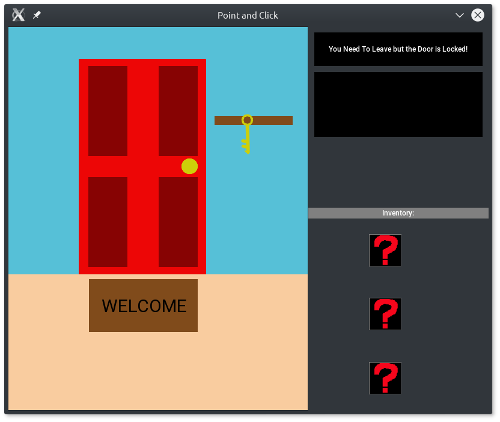
\includegraphics{Ch4-1}
\caption{Our Point-and-Click Game}
\end{figure}

The concept I chose for our game is like a super simple version of the "escape the room" puzzle games. You see a door and need to escape. If you are following along, give the game a try before you begin. It's Chapter4-1.py from Github. When writing out this code, feel free to use my (amazing) artwork if you don't fancy drawing anything yourself. 

\lstinputlisting[language=Python, caption=Our Game, captionpos=b]{Code/Chapter4-1.py} 

\subsection{GameScreen}

The  \lstinline[columns=fixed]{GameScreen Class} is essentially a nice container around the attributes associated with each screen. It holds a reference to our main \lstinline[columns=fixed]{Game} object, the image to display for this screen (I'll cover \lstinline[columns=fixed]{PhotoImage}s next), the region-of-interest (i.e. where to click in order to advance), an item to be picked up, and the help text to display. The \lstinline[columns=fixed]{on_click} function is sent the click event from the \lstinline[columns=fixed]{Game}'s \lstinline[columns=fixed]{Canvas}. It compares the coordinates of the clicked point of the \lstinline[columns=fixed]{Canvas} to its region-of-interest, then advances the game if the correct area was clicked. If the screen holds an inventory item it is added to the \lstinline[columns=fixed]{Game}'s inventory before advancing. I debated with myself whether or not to handle this logic within the \lstinline[columns=fixed]{Game} itself, but have decided it looks a bit neater here. 

\subsection{Game}
Our \lstinline[columns=fixed]{Game} object defines the main window and layout, as well as handles tracking and progressing in the game. Let's break it down a bit:

\subsubsection{\_\_init\_\_}

We begin with creating some empty \lstinline[columns=fixed]{list}s for our inventory and used-inventory (more on this later). We initialise the current screen to 0 and create a \lstinline[columns=fixed]{Font} which will be used to display a success message when the player finishes the game. After setting the title and size of the window, we also set \lstinline[columns=fixed]{resizable} to (False, False) to prevent the window from being resized in either direction. This removes any need to re-size the \lstinline[columns=fixed]{GameScreen} images if the player decides to change the window dimensions.

\vspace{5mm}

Next we create two \lstinline[columns=fixed]{PhotoImage} objects. These are just \lstinline[columns=fixed]{tkinter}'s way of holding an image file in a usable format. These \lstinline[columns=fixed]{PhotoImage}s can be placed onto widgets such as \lstinline[columns=fixed]{Button}s, \lstinline[columns=fixed]{Label}s and \lstinline[columns=fixed]{Canvas}es. These two \lstinline[columns=fixed]{PhotoImage}s will be going on \lstinline[columns=fixed]{Button}s which will represent our player's inventory. 

\vspace{5mm}      

We define a \lstinline[columns=fixed]{Canvas} and \lstinline[columns=fixed]{Frame} with fixed widths and heights which allows us to accurately split our screen in two. We use \lstinline[columns=fixed]{pack_propagate(0)} to keep the \lstinline[columns=fixed]{Frame} at its defined size. \lstinline[columns=fixed]{Frame}s will shrink to the size necessary to hold their contents by default, but we need this one to stay full-sized irrespective of its children.

\vspace{5mm}

We go on to define a \lstinline[columns=fixed]{StringVar} to hold our help text, a \lstinline[columns=fixed]{Label} to display it, another \lstinline[columns=fixed]{Label} to title our inventory, and a second \lstinline[columns=fixed]{Frame} inside the \lstinline[columns=fixed]{right_frame} to hold our inventory items. Our three inventory items are just \lstinline[columns=fixed]{Button}s which start off showing a question mark image. These are then \lstinline[columns=fixed]{pack}ed with some padding to space them out a bit. A \lstinline[columns=fixed]{tuple} is used to define (above,below) padding independently (which would be (left,right) inside \lstinline[columns=fixed]{padx}). We stick our inventory items into our \lstinline[columns=fixed]{inventory_slots} list and finish \lstinline[columns=fixed]{pack}ing before binding a method to left-clicking our canvas.

\subsubsection{Handling Game Screens}

\lstinline[columns=fixed]{set_game_screens} simply sets a list of \lstinline[columns=fixed]{GameScreen} objects as an attribute of our \lstinline[columns=fixed]{Game}. The reason this isn't in \lstinline[columns=fixed]{__init__} is because we need a reference to the \lstinline[columns=fixed]{Game} to create the \lstinline[columns=fixed]{GameScreens}. 

\vspace{5mm}

\lstinline[columns=fixed]{display_screen} takes in an index of our \lstinline[columns=fixed]{game_screens list} and keeps a reference to the \lstinline[columns=fixed]{GameScreen} at that index. It then clears the \lstinline[columns=fixed]{Canvas} and draws our current screen's image onto it. Finally it updates the help \lstinline[columns=fixed]{Label}'s \lstinline[columns=fixed]{StringVar} to display its hint to the player.

\vspace{5mm}

\lstinline[columns=fixed]{show_next_screen} updates the number which points to our current screen then checks that it is within the bounds of our \lstinline[columns=fixed]{game_screens}. If it is then we display the screen at that index. If it's not then we are out of screens, indicating that the player has won. In this case we set the \lstinline[columns=fixed]{Canvas} to black and show a success message. 

\subsubsection{Handling Inventory}

With this iteration of our inventory system, we're using a \lstinline[columns=fixed]{list} to track which slots are available. The length of the \lstinline[columns=fixed]{inventory_slots_in_use list} is used to select the next index of our inventory to add a new item to. The same check as \lstinline[columns=fixed]{show_next_screen} is used to ensure we are using a valid index of our \lstinline[columns=fixed]{inventory_slots} list, and if so the \lstinline[columns=fixed]{Button} at that slot is chosen. We \lstinline[columns=fixed]{configure} the \lstinline[columns=fixed]{Button} with the appropriate \lstinline[columns=fixed]{PhotoImage} for the item being added (in this case we just have the key) and append the \lstinline[columns=fixed]{item_name} to our \lstinline[columns=fixed]{inventory_slots_in_use list} to track that this slot is now in use. 

\subsection{Playing the Game}

We begin by making a \lstinline[columns=fixed]{Game} object as the main window. We then create three \lstinline[columns=fixed]{GameScreens} with their associated image, region-of-interest, item, and hint. The \lstinline[columns=fixed]{GameScreen}'s region-of-interest is specified as a 4-tuple with the first two numbers as the top-left x and y, and the second two as the bottom right x and y, forming a rectangle. We merge these together into a \lstinline[columns=fixed]{list} and pass it to our \lstinline[columns=fixed]{Game} with \lstinline[columns=fixed]{set_game_screens}. We finish up by calling \lstinline[columns=fixed]{play()} to set the initial screen and \lstinline[columns=fixed]{mainloop()} to make the window visible.

\subsection{Next Iteration}

Next up we'll be refining the inventory system logic as well as showing the history of hints in the big space below the current one. 

\newpage

\section{Our Refined Point-and-Click game}

With this iteration our item system is more sophisticated. We can now click and use things from our inventory and specify scenes which require the use of an item to continue. Let's look at how this is done.

\lstinputlisting[language=Python, caption=Our Game With Working Inventory, captionpos=b]{Code/Chapter4-2-abridged.py}

\subsection{GameScreen}

We've now got a new argument for each screen, \lstinline[columns=fixed]{required_item}, which establishes whether or not we need to be using an item to advance to the next screen. We've added some new logic to \lstinline[columns=fixed]{on_click} to accommodate this. 

\vspace{5mm}

The method now takes an \lstinline[columns=fixed]{item_in_use} argument which represents the active inventory item (if any). First off, we return if the game is won, to prevent clicks on the "You Win" screen. We display a message to the user if they are trying to use an item on a screen which does not require one, or they are outside of the scene's region-of-interest. When inside the region-of-interest, we check that the \lstinline[columns=fixed]{item_in_use} matches the scene's \lstinline[columns=fixed]{required_item} and only advance the screen if so. The rest of the logic is the same as before. 

\subsection{Game}

\subsubsection{\_\_init\_\_}

We've added a few new attributes to the beginning of our \lstinline[columns=fixed]{__init__}. We have a font for the message letting a user know they cannot use their selected item, a string which will hold the item currently in use, and a boolean for whether or not the game has been won.

\vspace{5mm}

Afterwards we define three \lstinline[columns=fixed]{StringVar}s for our help history and 3 \lstinline[columns=fixed]{Label}s to hold them. We next need 3 frames to hold our inventory \lstinline[columns=fixed]{Button}s and associated \lstinline[columns=fixed]{Label}s. Our \lstinline[columns=fixed]{Button}s have had \lstinline[columns=fixed]{command}s added so that they will now use an item when clicked (method will be covered later). We then define three more \lstinline[columns=fixed]{StringVar}s and \lstinline[columns=fixed]{Label}s to display the name of each item next to its button. The \lstinline[columns=fixed]{StingVar}s are put into a \lstinline[columns=fixed]{list} for access later. We finish off by \lstinline[columns=fixed]{pack}ing everything. 

\subsubsection{Handling Game Screens}

\lstinline[columns=fixed]{display_screen} is mostly the same, but now calls a new method \lstinline[columns=fixed]{show_help_text} instead of directly manipulating the \lstinline[columns=fixed]{help_var}.

\vspace{5mm}

\lstinline[columns=fixed]{show_next_screen} clears the used item when updating the screen, and sets \lstinline[columns=fixed]{has_won} to \lstinline[columns=fixed]{True} if the game has displayed all of its screens. 

\vspace{5mm}

The aforementioned \lstinline[columns=fixed]{show_help_text} propagates the values of each of our \lstinline[columns=fixed]{help_history StringVar}s down to the next one before setting the main \lstinline[columns=fixed]{help_var}'s text to that of the current \lstinline[columns=fixed]{GameScreen}.

\subsubsection{Handling the Inventory}

This is where the majority of changes this iteration are. Our \lstinline[columns=fixed]{add_inventory_item} method now grabs the \lstinline[columns=fixed]{StringVar} in the same index as the next open inventory slot and adds the name of the item to it. The \lstinline[columns=fixed]{.title()} here just capitalises the text for aesthetic purposes. 

\vspace{5mm}

Our new \lstinline[columns=fixed]{use_item} method (which is bound to each \lstinline[columns=fixed]{Button} in our inventory space) takes in the index of each inventory item as \lstinline[columns=fixed]{item_number}, checks it's valid for the size of the \lstinline[columns=fixed]{inventory_slots_in_use list} and sets it as our \lstinline[columns=fixed]{item_in_use}, which is used by our \lstinline[columns=fixed]{GameScreen}'s \lstinline[columns=fixed]{on_click}. It then loops through our inventory \lstinline[columns=fixed]{Button}s resetting them to a black background before configuring the clicked \lstinline[columns=fixed]{Button} to have a white background, indicating that the item is in use. It also swaps out the \lstinline[columns=fixed]{Button}'s \lstinline[columns=fixed]{command} to \lstinline[columns=fixed]{clear_used_item} so that the user can un-set the item if they want to deactivate it. 

\vspace{5mm}

Speaking of which, our \lstinline[columns=fixed]{clear_used_item} method sets our \lstinline[columns=fixed]{item_in_use} to an empty string, resets each \lstinline[columns=fixed]{Button}'s background to black and re-binds it's \lstinline[columns=fixed]{command} to its previous \lstinline[columns=fixed]{use_item}. We need to use a \lstinline[columns=fixed]{partial} from the \lstinline[columns=fixed]{functools} module to ensure we bind a function with the correct \lstinline[columns=fixed]{item_number} argument for each \lstinline[columns=fixed]{Button}.

\vspace{5mm}

If the player is trying to use an item somewhere in the scene where it is not usable, we need to tell them so. We do this with the \lstinline[columns=fixed]{show_cannot_use_message} method. This method creates some text on our \lstinline[columns=fixed]{Canvas} with our previously-defined font style. Since the \lstinline[columns=fixed]{create_text} method returns a unique ID for the created text, we store that in a variable called \lstinline[columns=fixed]{text_id}. We then use tkinter's \lstinline[columns=fixed]{after} method to schedule a function to be called after 2 seconds. This function is a \lstinline[columns=fixed]{lambda} which deletes the previously-created text by passing its ID to \lstinline[columns=fixed]{delete}. This ensures the text does not stay on the player's screen for the rest of that scene. 

\subsubsection{Playing the Final Game}

Just one change here - we pass the \lstinline[columns=fixed]{"key"} as the \lstinline[columns=fixed]{required_item} to our second scene. This means the player needs to activate the key in their inventory to open the door. 

\vspace{5mm}

This is where we will leave development of our point-and-click game. The fundamentals of just clicking a region and collecting / using items leads to the potential for a lot of gameplay. A lot of further development would require creating scenes and artwork, which has always been my weakpoint with game development. Despite this I feel like this point-and-click framework has a lot of potential, and is especially interesting given that it is written without an actual game engine. 

\subsection{Further Development}

If you'd like to continue work on this project as an exercise, try the following:

\begin{itemize}
  \item Add a screen which gives the player another item, and a screen which requires this item (how about it's raining outside so the player must pick up an umbrella?).
  \item Add cutscenes with dialogue boxes which can be advanced by pressing the space bar.
  \item Add a clues section which has a button for one clue per screen.
\end{itemize} 

\chapter{Ini File Editor}
In this chapter we'll be creating an app which allows us to edit \lstinline[columns=fixed]{.ini} config files. There's a folder in the code repository called \lstinline[columns=fixed]{ini_files} with a test file for you to play with while writing out this code. With this project we will learn about the following:

\begin{itemize}
  \item The \lstinline[columns=fixed]{Listbox} widget.
  \item The \lstinline[columns=fixed]{Spinbox} widget.
  \item Creating a file open and file save dialogue.
  \item Using keyboard shortcuts with \lstinline[columns=fixed]{Menu} items.
\end{itemize} 

\section{Basic View and Edit Functionality}

\begin{figure}[h]
\centering
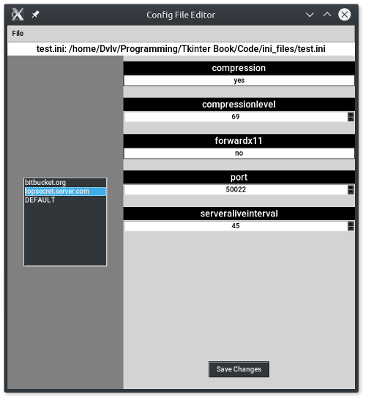
\includegraphics{Ch5-1}
\caption{Our Ini File Editor}
\end{figure}

\newpage

\lstinputlisting[language=Python, caption=Our Ini Editor, captionpos=b]{Code/Chapter5-1.py} 

\subsection{\_\_init\_\_}

We begin with the hopefully-now-familiar activities such as setting the window title and size, initialising some blank variables, creating our necessary widgets and packing everything. The \lstinline[columns=fixed]{active_ini} will hold our parsed \lstinline[columns=fixed]{.ini} file, the \lstinline[columns=fixed]{active_ini_filename} will hold the name of the given \lstinline[columns=fixed]{.ini} file, and \lstinline[columns=fixed]{ini_elements} will be used to associate a setting with a \lstinline[columns=fixed]{tkinter} widget. 

\vspace{5mm} 

We go on to create a \lstinline[columns=fixed]{Menu} containing a "file" option which holds "open" and "save" functionality. The \lstinline[columns=fixed]{accelerator} argument passed to the file options is used to display the keyboard shortcut which will activate them. 

\vspace{5mm}

Our window will be split into two \lstinline[columns=fixed]{Frame}s with the left being half as big as the right. We again use \lstinline[columns=fixed]{pack_propagate(0)} to stop them shrinking. We will also display a \lstinline[columns=fixed]{Label} at the top of the window telling the user which file they have open. We specify the \lstinline[columns=fixed]{font} argument here to increase the font size. The \lstinline[columns=fixed]{font} argument takes a tuple of three: (family, size, style). We can omit the family and style to have the font retain the defaults, and just give the size to make it bigger. This is why we use a tuple of \lstinline[columns=fixed]{(None, 12)} to modify only the size to 12.

\vspace{5mm}

Now that the layout is sorted, we create the only widget going into our left \lstinline[columns=fixed]{Frame} - the \lstinline[columns=fixed]{Listbox}. A listbox is somewhat like an expanded dropdown list. It displays multiple elements in a box and allows a user to select them. In this case we only want one selection at a time, so we set the \lstinline[columns=fixed]{selectmode} to \lstinline[columns=fixed]{tk.SINGLE} to enforce this. We then use \lstinline[columns=fixed]{exportselection=False} to prevent the selection from being "lost" when another widget is clicked. We \lstinline[columns=fixed]{pack} it up then bind a method to \lstinline[columns=fixed]{<<ListboxSelect>>} so that we can fire off an event when the user selects an option. 

\vspace{5mm}

After \lstinline[columns=fixed]{pack}ing our \lstinline[columns=fixed]{Frame}s we bind the keyboard shortcuts we added to our \lstinline[columns=fixed]{Menu} items to the same functions. With that, our \lstinline[columns=fixed]{__init__} is complete.

\subsection{file\_open}
Our \lstinline[columns=fixed]{file_open} method makes use of \lstinline[columns=fixed]{tkinter}'s \lstinline[columns=fixed]{filedialog} which takes care of opening files for us. The \lstinline[columns=fixed]{askopenfilename} method pops up a window with which the user can select a file and returns the path of this file, which we store in \lstinline[columns=fixed]{ini_file}. If the given filename does not end with ".ini" we show an error message and bring the open window back up again. We also need to check in this loop condition that \lstinline[columns=fixed]{ini_file} is not empty, so that the user can use the "cancel" option to end the interaction. If the filename is valid, we pass it off over to \lstinline[columns=fixed]{parse_ini_file}. 

\subsection{parse\_ini\_file}
We begin by creating an instance of a \lstinline[columns=fixed]{ConfigParser} which is a library that will handle parsing of \lstinline[columns=fixed]{.ini} files into almost-dictionaries. We store this object as \lstinline[columns=fixed]{self.active_ini} so that we can refer to it later, then tell it to read and parse the string we got from the file open dialogue. We also store the file path in \lstinline[columns=fixed]{self.active_ini_filename} so that we can write to the same file later on. 

\vspace{5mm}

After opening the file we need to clear any widgets which may still be in our \lstinline[columns=fixed]{right_frame}. If we don't do this the user would still see the first file's contents after opening a second, which would be confusing, and could lead to data loss if they then saved. We achieve this by using \lstinline[columns=fixed]{winfo_children} to get all children of the \lstinline[columns=fixed]{right_frame} and then calling \lstinline[columns=fixed]{destroy} on each to remove it.

\vspace{5mm}

Our job now is to get the sections of the file into our \lstinline[columns=fixed]{Listbox}. We begin by clearing the \lstinline[columns=fixed]{Listbox} in case there are any items left in there from previous file openings. We then \lstinline[columns=fixed]{enumerate} over our \lstinline[columns=fixed]{.ini} file's sections and \lstinline[columns=fixed]{insert} each into our \lstinline[columns=fixed]{Listbox}. Since the "DEFAULT" section is not returned by the call to \lstinline[columns=fixed]{sections()} we manually account for it afterwards if it exists. We finish up by putting the filename at the top of the window in our \lstinline[columns=fixed]{file_name_label}. We use \lstinline[columns=fixed]{ntpath} to parse the file name out of the path string, then put a colon, followed by the full path string. Now that our \lstinline[columns=fixed]{Listbox} is populated we can display the contents of a section to the user once they have selected one.

\subsection{display\_section\_contents}

We first need to check we have an \lstinline[columns=fixed]{.ini} file to work with, and show an error message if not. We follow on by clearing out the contents of our right \lstinline[columns=fixed]{Frame} to ensure it is empty, and then do the same for our dictionary of ini elements. We now need to populate our \lstinline[columns=fixed]{Frame} with the elements in the chosen ini section.

\vspace{5mm}

The currently selected \lstinline[columns=fixed]{Listbox} element is grabbed by passing the id returned by \lstinline[columns=fixed]{curselection()} to its \lstinline[columns=fixed]{get()} method. Next we iterate over a sorted version of the chosen section in our parsed \lstinline[columns=fixed]{.ini} file and create a \lstinline[columns=fixed]{Label} with the item's name. The item's value is grabbed using the current \lstinline[columns=fixed]{key} and its type is checked. If it's a number, we create a \lstinline[columns=fixed]{Spinbox}, otherwise we use a normal \lstinline[columns=fixed]{Entry}. The numerical \lstinline[columns=fixed]{Spinbox} utilises an \lstinline[columns=fixed]{IntVar} (like a \lstinline[columns=fixed]{StringVar} for integers) to set its default value to the one read from the ini file. We use the \lstinline[columns=fixed]{from_} and \lstinline[columns=fixed]{to} arguments to set the minimum and maximum values we can spin to. 

\vspace{5mm}

We finish off by \lstinline[columns=fixed]{pack}ing our chosen element and then pairing it with the \lstinline[columns=fixed]{key} in our \lstinline[columns=fixed]{ini_elements} dictionary. This allows us to keep track of which widget's value should be associated to which config item when saving. Speaking of saving, we also create a \lstinline[columns=fixed]{Button} to save without going up into the \lstinline[columns=fixed]{Menu}. 

\subsection{file\_save}

Before we attempt to save we again check to make sure we have a loaded \lstinline[columns=fixed]{.ini} file to write to. We then get the chosen section from our \lstinline[columns=fixed]{Listbox} and iterate over the section's items. We set each item's value to the value of its associated widget. We finish up by opening the file at the location stored in \lstinline[columns=fixed]{active_ini_filename} and telling our \lstinline[columns=fixed]{ConfigParser} to write into it. We finally display a message to let the user know that the file has been saved. 

\subsection{Next Iteration}

The user currently has to save each section before loading the next one, otherwise any changes will be lost. We'll look at adjusting our \lstinline[columns=fixed]{ini_elements} to hold all of the changed values until the program is closed. There's also some graphical tweaks we need to make to better handle the screen resizing. 

\newpage

\section{Now With Caching and Resizing}

With this iteration we hold the updated values in memory even when switching between sections. This means the user can update as many sections as they want and will only need to save once at the end. We've also updated the size of the \lstinline[columns=fixed]{Frame}s on re-size. Let's take a look at how this is done:

\lstinputlisting[language=Python, caption=Our Ini Editor, captionpos=b]{Code/Chapter5-2-abridged.py} 

\subsection{\_\_init\_\_ and frame\_height}

We've now removed the fixed heights from our \lstinline[columns=fixed]{Frame}s and bound a method to their \lstinline[columns=fixed]{<Configure>} event. This method gets the root window's height and sets the height of the right \lstinline[columns=fixed]{Frame} to the same value. The left \lstinline[columns=fixed]{Frame} also follows suit. Now when the user re-sizes the window the \lstinline[columns=fixed]{Frames} will adjust accordingly. Horizontal adjustment was already handled by the \lstinline[columns=fixed]{expand=1} on our right \lstinline[columns=fixed]{Frame}'s \lstinline[columns=fixed]{pack}.

\vspace{5mm}

We have also used the \lstinline[columns=fixed]{anchor} argument when packing our \lstinline[columns=fixed]{file_name_label} to fix it to the very top of the screen.  

\subsection{parse\_ini\_file}

Since we need to keep track of each individual section's items, we now create an attribute for each section in our \lstinline[columns=fixed]{ini_elements} dictionary, which is initialised as another empty dictionary. This will be written to with \lstinline[columns=fixed]{display_section_contents}.

\subsection{display\_section\_contents}

I've left this entire method in for clarity, but some has stayed the same. We now unpack the widgets associated with each section instead of \lstinline[columns=fixed]{destroy}ing them so that we can retain a reference to their values. \lstinline[columns=fixed]{pack_forget} removes widgets from their parent but does not destroy them in memory, meaning we can remove them from the frame without losing their values. 

\vspace{5mm}

Within our loop we now check to see if we have elements for the chosen section already. If we do we grab them, otherwise we stick an empty dictionary into our \lstinline[columns=fixed]{section_elements} variable to trigger our second \lstinline[columns=fixed]{except} block. If we have the element already, we grab it out of \lstinline[columns=fixed]{ini_elements} and pack it, otherwise we create it, put it into \lstinline[columns=fixed]{ini_elements}, and set the default just as before (except now each element is under the key of its section name). We use \lstinline[columns=fixed]{try} and \lstinline[columns=fixed]{except} to catch \lstinline[columns=fixed]{KeyError}s here as a way of testing whether or not the elements are already loaded in our cache (\lstinline[columns=fixed]{ini_elements}) rather than as a way of handling something "going wrong". You may know the python idiom "it's easier to ask forgiveness than permission" which is what we have applied here. Instead of trying to check whether or not the ini element has been loaded, we simply assume it has and handle the resulting \lstinline[columns=fixed]{KeyError} if it hasn't.

\subsection{file\_save}

Since we now store each element inside the key of its section, we simply iterate over each section and update the \lstinline[columns=fixed]{active_ini} accordingly. 

\subsection{Running}

Nothing has changed with regards to running this iteration. You should be able to launch it as before. You can now try changing some of the values under one section, then swapping to a different section and back to the first, and you should see the changes you made have persisted. 

\subsection{Next Iteration}
With our current app we can edit existing content but cannot create anything new. We will finish this project off with the ability to create new .ini files, new sections and new items.

\newpage

\section{Our finished Ini Editor}
Now complete with creating capabilities, let's look at our finalised app:

\lstinputlisting[language=Python, caption=Our Ini Editor, captionpos=b]{Code/Chapter5-3-abridged.py} 

\subsection{CentralForm}
To save a bunch of \lstinline[columns=fixed]{__init__} method duplication we've got a base-class for a form which will appear in the center of its parent window. The \lstinline[columns=fixed]{__init__} method begins by grabbing the x and y co-ordinates of its master (our IniEditor instance) as well as its width and height. It then has variables representing its own width and height which it uses to calculate where to place itself in order to be in the center of the master and stores these in \lstinline[columns=fixed]{pos_x and pos_y}. It finally calls the \lstinline[columns=fixed]{.geometry()} method on a formatted string of (width x height + x + y) to define its size and position in one go. Now we have this we can create other windows which inherit from this class, and as long as they call \lstinline[columns=fixed]{super().__init__(master)} they will be placed in the center of their master. Let's look at our 2 child classes now.

\subsection{AddSectionForm and AddItemForm}
Both of these windows initialise by creating and packing some \lstinline[columns=fixed]{Label}s and \lstinline[columns=fixed]{Entries} followed by a submit \lstinline[columns=fixed]{Button}. Both then have a method attached to their \lstinline[columns=fixed]{Button} which grabs the values from the \lstinline[columns=fixed]{Entries} and sends them over to the master if they aren't blank. When showing the error \lstinline[columns=fixed]{messagebox} we specify the parent as \lstinline[columns=fixed]{self} to ensure that it displays on top of our forms. Since the forms and \lstinline[columns=fixed]{messagebox}es both display in the center of the master, our error message would appear behind our forms since by default they are parented to the main \lstinline[columns=fixed]{Tk} object. By passing in the \lstinline[columns=fixed]{parent} argument as \lstinline[columns=fixed]{self} we ensure they appear in front of our form. We don't need to do this on success as we destroy the form object beforehand anyway. 

\subsection{IniEditor}

\subsubsection{\_\_init\_\_ and file\_new}

We've now added a "new" option to our file menu and given it a keyboard shortcut. These both call our \lstinline[columns=fixed]{file_new} method. This method uses the \lstinline[columns=fixed]{asksaveasfilename} method of the \lstinline[columns=fixed]{filedialog} to grab a filename from the user, which must end in .ini as before, and then parses it. We've passed in the \lstinline[columns=fixed]{filetypes} argument to force the file to end with \lstinline[columns=fixed]{.ini} this time (and done the same in \lstinline[columns=fixed]{file_open} too). Even thought this new file will be blank, passing it to our \lstinline[columns=fixed]{parse_ini_file} method still sets it up in our \lstinline[columns=fixed]{active_ini} and \lstinline[columns=fixed]{active_ini_filename} variables, as well as putting the filename at the top of our window. 

\subsubsection{Adding items and sections}

Our \lstinline[columns=fixed]{add_*_form} methods both just create an instance of the relevant form windows, which then in turn call their \lstinline[columns=fixed]{add_*} methods on the master. Our \lstinline[columns=fixed]{add_section_form} needs to check there is an .ini file open before running, but our \lstinline[columns=fixed]{add_item_form} doesn't need to as the \lstinline[columns=fixed]{Button} won't be rendered without an open file. 

\vspace{5mm}

\lstinline[columns=fixed]{add_section} simply adds a new empty dictionary into our \lstinline[columns=fixed]{active_ini} with the key matching the text entered into the form. It then calls a new method - \lstinline[columns=fixed]{populate_section_select_box} - which clears and re-populates the \lstinline[columns=fixed]{Listbox}. It's moved into its own method since we now do this in two places.

\vspace{5mm}

\lstinline[columns=fixed]{add_item} is similar - but it needs to get the current section from our \lstinline[columns=fixed]{Listbox}, and then add a key-value pair to it's dictionary. We then call \lstinline[columns=fixed]{display_section_contents} so that the new item appears on the users screen right away and we get its widget into our cache for saving.

\subsubsection{display\_section\_contents}

The only change here is to add the "Add Item" \lstinline[columns=fixed]{Button} which calls \lstinline[columns=fixed]{add_item_form}. Even though we \lstinline[columns=fixed]{pack} this after our \lstinline[columns=fixed]{save_button} it will appear above it, due to the use of \lstinline[columns=fixed]{tk.BOTTOM}.

\vspace{5mm}

That's it for development of our \lstinline[columns=fixed]{.ini} file editor. We now have an application which allows us to change specific values without having to wade through the large blocks of comments often written in \lstinline[columns=fixed]{.ini} files. Along the way we've learned how to use \lstinline[columns=fixed]{Listbox}es to allow the user to make choices which affect the GUI, and \lstinline[columns=fixed]{Spinbox}es to allow for precision when adjusting numbers. No more typos when trying to increase a 2 to a 3 and ending up with 23 instead!

\subsection{Further Development}

If you'd like to continue work on this project as an exercise, try the following:

\begin{itemize}
  \item Make the right \lstinline[columns=fixed]{Frame} scrollable using a \lstinline[columns=fixed]{Canvas} (remember chapter 2?).
  \item Alter the running code to allow the user to launch the application with a specific file from the command line, such as "\lstinline[columns=fixed]{python inifileeditor.py test.ini}"
  \item Add deletion functionality to complete all 4 parts of CRUD (Create, Read, Update, Delete). 
\end{itemize} 

\chapter{A Python Text Editor With Autocomplete and Syntax Highlighting}
In this chapter we'll be making a simple Python editor complete with syntax highlighting and some basic auto-completion. Here we'll learn about:

\begin{itemize}
  \item More advanced features of the \lstinline[columns=fixed]{Text} widget.
  \item More advanced event binding.
  \item Using \lstinline[columns=fixed]{Menu}s outside of a top bar.
  \item Using tags.
  \item Overriding some of the window manager's event calls.
\end{itemize}

\section{Basic Functionality and Autocompletion}

\begin{figure}[h]
\centering
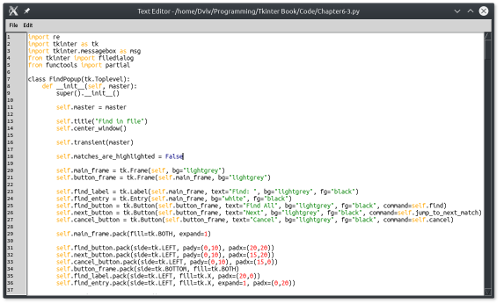
\includegraphics{Ch6-3}
\caption{Our Text Editor.}
\end{figure}

\newpage

\lstinputlisting[language=Python, caption=Text Editor, captionpos=b]{Code/Chapter6-1.py}

\subsection{\_\_init\_\_}

We begin with some constants. \lstinline[columns=fixed]{FONT_SIZE} will be used to adjust the positioning of the autocomplete menu (and also the font size used in our editor, as you probably guessed). Next is the \lstinline[columns=fixed]{AUTOCOMPLETE_WORDS} list which holds all of the words which we wish to autocomplete. Finally is the self-explanitory \lstinline[columns=fixed]{WINDOW_TITLE}. We also define \lstinline[columns=fixed]{open_file} which will be a string representing the path of our currently opened file (much like last chapter) then set the title and geometry.

\vspace{5mm}

We then move on to our menu bar, which is much the same as the one from last chapter. We create the new, open, and save buttons which are fairly standard for text editors.

\vspace{5mm}

The last thing we need is the main area to enter text, which is achieved using a \lstinline[columns=fixed]{Text} widget. We specify the colours and the font (if you don't have ubuntu mono feel free to change this) and \lstinline[columns=fixed]{pack} it to take up as much space as it can with \lstinline[columns=fixed]{expand=1} and \lstinline[columns=fixed]{fill=tk.BOTH}. We finish up by binding some methods to space, tab, and KeyRelease (each will be covered below) as well as the open, new, and save bindings from our \lstinline[columns=fixed]{file_menu}.

\subsection{Handling Files}

\lstinline[columns=fixed]{file_new} sets the value of our \lstinline[columns=fixed]{open_file} to the one returned by \lstinline[columns=fixed]{asksaveasfilename} and empties our \lstinline[columns=fixed]{Text} area before changing the window title to display the new file's path.

\vspace{5mm}

\lstinline[columns=fixed]{file_open} uses \lstinline[columns=fixed]{askopenfilename} to grab an existing file name and sets it as our \lstinline[columns=fixed]{open_file}. It then clears the contents of our \lstinline[columns=fixed]{Text} area to get rid of any existing text in there. Afterwards the file is opened in read mode and we obtain a list of each line with \lstinline[columns=fixed]{readlines()}. Each line is \lstinline[columns=fixed]{insert}ed into our \lstinline[columns=fixed]{Text} area at the relevant index. We add 1.0 to the float value of the \lstinline[columns=fixed]{list} index because \lstinline[columns=fixed]{tkinter}'s indexing starts at 1.0, whereas python's \lstinline[columns=fixed]{list} indexing begins at 0. We then finish by displaying the open file in the window's title as before.

\vspace{5mm}

\lstinline[columns=fixed]{file_save} begins by checking if we have an \lstinline[columns=fixed]{open_file}, and if not will try and get one with \lstinline[columns=fixed]{asksaveasfilename()}. If that was successful, we grab the text out of our \lstinline[columns=fixed]{Text} area and write it into our opened file.

\subsection{Autocompletion}

\subsubsection{display\_autocomplete\_menu}

We'll start off with \lstinline[columns=fixed]{display_autocomplete_menu} which is bound to \lstinline[columns=fixed]{<KeyRelease>}, meaning it's called every time a key is typed into our \lstinline[columns=fixed]{Text} area. We begin by grabbing the current index of the cursor with \lstinline[columns=fixed]{index(tk.INSERT)}. This is returned in a string of the format "x.y". For example, the first character of the second line is "1.2" and the 14th character of line 12 is "14.12". The reason we need this is to try and grab the word which is currently being typed by the user. We need to go back one character in order to do this, which is where \lstinline[columns=fixed]{adjust_floating_index} comes in. In \lstinline[columns=fixed]{adjust_floating_index} we split off the string on the point to get the x and y indices. Then we need to remove 1 from \lstinline[columns=fixed]{y_index} and put it back together as a string in the form of "x.y". With this done, we can use \lstinline[columns=fixed]{tkinter}'s magic word "wordstart" to get the beginning of the word being typed. This is combined with the \lstinline[columns=fixed]{INSERT} position of the cursor to grab the \lstinline[columns=fixed]{currently_typed_word}. This may be hard to grasp, so here's a picture which will hopefully clear it up a bit:

\begin{figure}[h]
\centering
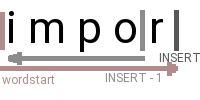
\includegraphics{Ch6-ws}
\caption{Finding our current word boundaries. Word is the pink arrow.}
\end{figure}

\vspace{5mm}

Now that we have the currently typed word (or not, if there was a TclError raised along the way due to a bad index) we begin by destroying the autocomplete menu if it is already active, since we will only want one up at a time, and then we build a \lstinline[columns=fixed]{list} of suggestions based on the current word. We do this by looping through our \lstinline[columns=fixed]{AUTOCOMPLETE_WORDS} and \lstinline[columns=fixed]{append}ing ones which start with what the user is currently typing (but not any which are equal to it, since then there's no need to "complete" what they've already typed). If there are any matching suggestions then we need to show the menu. We get the coordinates with \lstinline[columns=fixed]{get_menu_coordinates} (covered next) and instantiate a new \lstinline[columns=fixed]{Menu} to hold each suggestion.

\vspace{5mm}

We loop through each suggestion and create a \lstinline[columns=fixed]{partial} of \lstinline[columns=fixed]{insert_word} (covered below) passing in the suggested word, the currently-being-typed word and the index of our cursor. We then add a menu item for this word with the \lstinline[columns=fixed]{partial} as its command. After all suggestions are added, we use \lstinline[columns=fixed]{post(x, y)} to place our menu exactly at the calculated coordinates and bind the down arrow key so that it focuses the first menu item.

\subsubsection{get\_menu\_coordinates}
In order to calculate where to put our autocomplete menu we use the \lstinline[columns=fixed]{Text} area's \lstinline[columns=fixed]{bbox} method to get the bounding box of the cursor position (\lstinline[columns=fixed]{tk.INSERT}). We then add on the x and y position of our main window to ensure it displays within the application itself, and add some extra onto the y so that our menu doesn't cover up what the user is currently typing.  

\subsubsection{insert\_word}
In order to complete the word being typed, we need to know how much has already been entered. We get this with \lstinline[columns=fixed]{len(part)} and use it to get the rest of the word which needs to be inserted. We then need to build another of \lstinline[columns=fixed]{tkinter}'s magic strings to tell it how many characters are being inserted. The format "+nc" implies n characters ahead of the given index, so "+2c" goes 2 characters forward.

\vspace{5mm}

With all of that figured out we insert the rest of the word at the current cursor's position and then move the cursor forward the appropriate number of characters with \lstinline[columns=fixed]{mark_set} so that it is at the end of the newly-completed word. We then \lstinline[columns=fixed]{destroy} the autocomplete menu and force the focus back to our \lstinline[columns=fixed]{Text} area so that the user can continue typing.

\subsubsection{Focusing and Destroying the Menu}

\lstinline[columns=fixed]{focus_menu_item} forces focus onto the autocomplete menu and sets its first item as active so the user can select it with Enter. If we somehow end up here with no menu (or an empty menu) then we will get a \lstinline[columns=fixed]{TclError}, which we can just ignore and do nothing.

\vspace{5mm}

\lstinline[columns=fixed]{destroy_autocomplete_menu} calls \lstinline[columns=fixed]{destroy} on our menu and unbinds the down arrow from our \lstinline[columns=fixed]{Text} area. If the menu doesn't exist then the \lstinline[columns=fixed]{TclError} is caught and nothing will happen. We finally force the focus back to our \lstinline[columns=fixed]{Text} area so that the user can continue typing. 

\subsection{Spaces over Tabs!?}

There's a method called \lstinline[columns=fixed]{insert_spaces} bound to the Tab key which inserts 4 spaces and uses \lstinline[columns=fixed]{return "break"} to prevent the default behaviour of said key. This is to demonstrate how to make an event binding override the default key behaviour. Using \lstinline[columns=fixed]{return "break"} we end the chain of events caused by pressing the Tab key, meaning no Tab character is inserted. Most editors will offer the option of inserting spaces when pressing Tab, and using 4 spaces conforms to PEP-8.
 
\subsection{Next Iteration}

Now it's time to utilise some \lstinline[columns=fixed]{tags} to get syntax highlighting working. 

\newpage

\section{Syntax Highlighting}
With this iteration we have some syntax highlighting for strings, numbers, decorators, and various language keywords. A lot of the code has stayed the same, just a small addition to \lstinline[columns=fixed]{file_open} to highlight files upon opening them. 

\lstinputlisting[language=Python, caption=Text Editor, captionpos=b]{Code/Chapter6-2-abridged.py}

\subsection{\_\_init\_\_}

We've got some more autocomplete words now as well as two more lists which separate them out a bit. This is to avoid colouring all keywords with the same colour, which looks horrible in my opinion. We then have a big pile of regexes which will match spaces, strings, numbers and keywords. I will try to explain each below. After that we've got a dictionary mapping the regexes to strings, which are some of the tag names defined below. We use \lstinline[columns=fixed]{tag_config} to define a tag represented by a string (the first argument) and add some styling associated with it (the proceeding keyword arguments). Anything which is given the tag "keyword1" will be orange, for example. 

\vspace{5mm}

A tag is essentially just a group of properties which can be assigned to certain characters within the \lstinline[columns=fixed]{Text} area. In this instance we are changing the colour of certain words to achieve syntax highlighting.

\vspace{5mm}

We've adjusted the method bound to \lstinline[columns=fixed]{<KeyRelease>} to a new one, since we now want to call 2 methods each time. This will be covered later. 

\subsection{Regexes Explained}

\lstinputlisting[language=Python, caption=Regex Explanations, captionpos=b]{Code/Chapter6-regex-explain.py}

\subsection{file\_open}

After all of the previous code for opening files, we need to run them through our \lstinline[columns=fixed]{tag_keywords} method to apply the syntax highlighting. Since this function works line-by-line, we get the index of the end of our file and split the x off of \lstinline[columns=fixed]{tkinter}'s "x.y" indexing format. This gives us the number of the last line, which is also the number of lines in the document. We can then iterate over the \lstinline[columns=fixed]{range} of that number, build a \lstinline[columns=fixed]{tkinter} index of "line\_number.0" and pass it into our \lstinline[columns=fixed]{tag_keywords} method. Speaking of which:

\subsection{tag\_keywords}

The main bulk of this iteration is right here. As mentioned, this method works on a line-by-line basis, so we need to check whether we have a line number passed in. If not, we use the line with the cursor on it. We again split off the x and join it with a 0 to get the \lstinline[columns=fixed]{tkinter} index of the line's beginning. We combine that with the magic word "lineend" within \lstinline[columns=fixed]{get} to get the contents of the whole line. We can then use \lstinline[columns=fixed]{split()} to get each individual "word" on the line. We grab the number of leading spaces on the line so that we can adjust our y position to the start of the actual text. 

\vspace{5mm}

With all of that set up, we remove all tags on the current line so that we can overwrite them with new ones. We do this by looping through all of our \lstinline[columns=fixed]{tag_names()} and calling \lstinline[columns=fixed]{tag_remove} on the entire line. Without this, when the user types "as" it will become highlighted because it is a keyword. If they then continue to write the full word "assumption" the first "as" will remain highlighted, which will look wrong and be offputting. 

\vspace{5mm}

The first thing to do is to add the regex-specified tags. Let's jump to that method now:

\subsubsection{add\_regex\_tags}

We iterate over our \lstinline[columns=fixed]{dictionary} of regex-to-tag mappings and use \lstinline[columns=fixed]{find_iter} over the current line to see if we have any matches. If we do, the \lstinline[columns=fixed]{span()} function handily gives us the start and end indexes of the entire string at which this match occcurs. We \lstinline[columns=fixed]{join} these to the line number with a dot to match \lstinline[columns=fixed]{tkinter}'s indexing and add the associated tag in that range. 

\subsubsection{back to tag\_keywords}

Now that we've covered the more complex cases we can do a slightly more manual approach to finish off the remaining keyword types. We strip off brackets, colons, and commas because they are part of some keywords (if:, else:) but we don't want them to be coloured. We then use the current y position as the word's start and add the length to it to get the word's end. We join it with the line number to get an index as usual so that we can begin comparison.  

\vspace{5mm}

All we have to do is check whether the word is in one of our keywords \lstinline[columns=fixed]{list}s, and if it is, assign the relevant tag to its range. We just use \lstinline[columns=fixed]{startswith("@")} to find a decorator for simplicity. We then update the current y position with the length of the word plus one (for the space character). 

\vspace{5mm}

That's all there is to applying the syntax highlighting to our \lstinline[columns=fixed]{Text} area. The majority of the work is figuring out how to correctly keep track of the relevant \lstinline[columns=fixed]{tkinter} index of the word you wish to colour. 

\subsubsection{Why Two Methods of Tagging?}

Certain keywords should not be observed as part of a bigger "word". Take "if" for example. It should generally appear by itself (aside from the colon, which we can easily strip off). Now consider "None". "None" will often get merged into a bigger "word". For example: \lstinline[columns=fixed]{self.add_task(None, task_text, True)}. Here there is no spacing around "None", which is the correct python styling, but when \lstinline[columns=fixed]{split}ting this line we get one big chunk of \lstinline[columns=fixed]{self.add_task(None,} which is not equal to "None". We can't pick out the "None" easily here, which is why we need to use regex. 

\vspace{5mm}

Strings and numbers are also different beasts entirely. You can't really build a list of all possible strings or numbers, so regex is a must in order to match them. 

\subsection{display\_autocomplete\_menu, number\_of\_leading\_spaces, and on\_key\_release}

\lstinline[columns=fixed]{display_autocomplete_menu} now has \lstinline[columns=fixed]{destroy_autocomplete_menu} bound to Escape so that the user can close it and continue typing. The same binding was added to our \lstinline[columns=fixed]{main_text} in \lstinline[columns=fixed]{__init__}. 

\lstinline[columns=fixed]{number_of_leading_spaces} is a method taken from an older project of mine. It uses a regex matching 0 or more space characters at the start of a string. If it finds a match, we return the length of the match, otherwise 0.

\vspace{5mm}

\lstinline[columns=fixed]{on_key_release} is just created to call two methods on the \lstinline[columns=fixed]{<KeyRelease>} event. It displays the autocomplete menu as before as well as updating our syntax highlighting tags with \lstinline[columns=fixed]{tag_keywords}. We do not want to display the autocomplete menu on a few specific key presses, including the arrow keys, backspace, and escape, so we will check the \lstinline[columns=fixed]{event.keysym} before calling \lstinline[columns=fixed]{display_autocomplete_menu}. \lstinline[columns=fixed]{event.keysym} returns a human-readable representation of the key which triggered the event. 

\subsection{Next Iteration}
We'll finish off our text editor by adding some standard features to bring it in line with other text editors, including a scroll bar, line numbers, select-all, find, and an Edit menu. 

\newpage

\section{Our Finished Editor}

\lstinputlisting[language=Python, caption=Our Finished Editor, captionpos=b]{Code/Chapter6-3-abridged.py}

\subsection{FindPopup}

\subsubsection{\_\_init\_\_}

After setting the title and borrowing code from our ini editor to center this window with the \lstinline[columns=fixed]{center_window} method, we specify that this window should be a \lstinline[columns=fixed]{transient}, which means it will remain over the top of our main window until closed. Next is a boolean which we use to indicate if the matches are highlighted in the main window or not. We then define two frames: a main one for the whole window and a button frame to hold our \lstinline[columns=fixed]{Button}s. We \lstinline[columns=fixed]{pack} our \lstinline[columns=fixed]{Label} and \lstinline[columns=fixed]{Entry} in the \lstinline[columns=fixed]{main_frame} and our three \lstinline[columns=fixed]{Button}s - Find All, Next, and Cancel - into the \lstinline[columns=fixed]{button_frame}, which is \lstinline[columns=fixed]{pack}ed to the bottom of the \lstinline[columns=fixed]{main_frame}. We force focus to the \lstinline[columns=fixed]{Entry} so that the user doesn't have to click in it to begin typing, bind Enter to our \lstinline[columns=fixed]{jump_to_next_match} method, bind Escape to our \lstinline[columns=fixed]{cancel} method, and override the window manager using \lstinline[columns=fixed]{self.protocol("WM_DELETE_WINDOW", <callback>)} so that our \lstinline[columns=fixed]{cancel} method will be called when the user closes the window. 

\subsubsection{The rest}

Our \lstinline[columns=fixed]{find} method sets the \lstinline[columns=fixed]{matches_are_highlighted} flag to \lstinline[columns=fixed]{True} to avoid repeatedly calling the \lstinline[columns=fixed]{highlight_matches} method of the master window, and calls \lstinline[columns=fixed]{highlight_matches} with the text from our \lstinline[columns=fixed]{Entry}, providing there is something written in there and the matches are not already highlighted. 

\vspace{5mm}

\lstinline[columns=fixed]{jump_to_next_match} will call \lstinline[columns=fixed]{find()} if the matches for the \lstinline[columns=fixed]{Entry}'s text are not currently highlighted, then pass off to the \lstinline[columns=fixed]{next_match} method of our master window. 

\vspace{5mm}

\lstinline[columns=fixed]{cancel} will tell the master window to remove the tags added by the find methods and then destroy our FindPopup instance. 

\vspace{5mm}

\lstinline[columns=fixed]{matches_are_not_highlighted} will set \lstinline[columns=fixed]{matches_are_highlighted} to \lstinline[columns=fixed]{False} if any key except Enter is pressed within our \lstinline[columns=fixed]{Entry}, as this indicates the word to search for has now changed and needs to be re-found. 

\vspace{5mm}

\lstinline[columns=fixed]{center_window} came from our Ini Editor, so see the previous chapter for an explanation.

\subsection{Editor}

\subsubsection{\_\_init\_\_}

With this iteration, we have an edit menu to accompany our file menu. It's created in the same way with \lstinline[columns=fixed]{cut, paste, undo,} and \lstinline[columns=fixed]{redo} buttons. 

\vspace{5mm}

Our line numbers are handled by a disabled \lstinline[columns=fixed]{Text} widget. It's six characters wide, meaning it can keep track of up to one million lines of code (I hope nobody ever encounters a million-line file however!) We start it off at line 1 and \lstinline[columns=fixed]{pack} it over to the left. 

\vspace{5mm}

We create a \lstinline[columns=fixed]{Scrollbar} and bind it to a command - \lstinline[columns=fixed]{scroll_text_and_line_numbers} - as it will need to scroll both of our \lstinline[columns=fixed]{Text} widgets simultaneously. We also pair the \lstinline[columns=fixed]{main_text}'s \lstinline[columns=fixed]{yscrollcommand} to the bar to ensure the bar moves when we scroll with the mouse. We \lstinline[columns=fixed]{pack} this to the right before finally packing our \lstinline[columns=fixed]{main_text} so that everything is in the right place.

\vspace{5mm}

We finish up by adding a new tag - findmatch - to indicate matches made from our FindPopup, and finally binding some key events.  

\subsubsection{Scrolling}

\lstinline[columns=fixed]{scroll_text_and_line_numbers} will receive different arguments depending on if it is triggered by the \lstinline[columns=fixed]{Scrollbar} or mouse wheel. The \lstinline[columns=fixed]{Scrollbar} will pass a tuple of ("moveto", <fraction>) over here, so we can directly call \lstinline[columns=fixed]{yview_moveto} and pass over the fraction argument. Our mouse wheel will only pass the usual event object which will raise an \lstinline[columns=fixed]{IndexError} if we try and grab element [1] from it. Therefore we catch this exception and use the code we saw in Chapter 2 to scroll both areas. 

\vspace{5mm}

Our \lstinline[columns=fixed]{skip_event} method is bound to the mouse wheel on the \lstinline[columns=fixed]{line_numbers}. This is to stop the user from scrolling the line numbers. The method just uses \lstinline[columns=fixed]{return "break"} in order to do nothing but end the chain of events triggered by scrolling. 

\subsubsection{select\_all, file\_open, and on\_key\_release}

Simple changes here. We want to update the line numbers after opening a file for obvious reasons, so we call \lstinline[columns=fixed]{update_line_numbers} (covered later). Same deal for \lstinline[columns=fixed]{on_key_release}. \lstinline[columns=fixed]{select_all} adds the \lstinline[columns=fixed]{"sel"} tag to all of the text in our \lstinline[columns=fixed]{main_text} area, thereby selecting it all. 

\subsubsection{The Edit Menu}

As well as binding callbacks to events in \lstinline[columns=fixed]{tkinter}, we can generate the events ourselves using \lstinline[columns=fixed]{event_generate}. Here we generate the \lstinline[columns=fixed]{<<Cut>>, <<Paste>>, <<Undo>>,} and \lstinline[columns=fixed]{<<Redo>>} events. 

\vspace{5mm}

After pasting we want to make sure the new text is syntax-highlighted. To do this we have abstracted some code from \lstinline[columns=fixed]{file_open} into a new function - \lstinline[columns=fixed]{tag_all_lines} - which we call after pasting. We also call \lstinline[columns=fixed]{on_key_release} directly, since we are returning \lstinline[columns=fixed]{"break"}, which will both update the line numbers and trigger auto-completion if we paste part of a keyword. We have bound \lstinline[columns=fixed]{<Control-v>} to this paste method in \lstinline[columns=fixed]{__init__} to ensure this happens when the user pastes from the keyboard shortcut too. 

\subsubsection{update\_line\_numbers}

In order to update the line numbers as the opened file grows, we enable our \lstinline[columns=fixed]{line_numbers} widget, remove all of its contents, grab the number of lines off of the end-of-file index, join each number in the \lstinline[columns=fixed]{range} up to our final line with a newline character, place this long string into the widget, and finally disable it again. Note that we add 1 to each line number in our loop. This is because we \textit{don't} want our first line to be line 0 and we \textit{do} want the last value included.

\subsubsection{highlight\_matches}

We begin this method by removing all "findmatch" tags from our \lstinline[columns=fixed]{main_text} widget and initialising a couple of variables which we will use to keep track of our matches. We then compile \lstinline[columns=fixed]{text_to_match}, which came from the \lstinline[columns=fixed]{Entry} in our FindPopup, as regex. This allows the user to put an actual regular expression in this box as well as the literal text. We then split the \lstinline[columns=fixed]{main_text}'s contents on newline characters to get a \lstinline[columns=fixed]{list} of every line. We \lstinline[columns=fixed]{enumerate} over this \lstinline[columns=fixed]{list} and use code very similar to that in our \lstinline[columns=fixed]{add_regex_tags} to add a "findmatch" tag to the relevant \lstinline[columns=fixed]{tkinter} index range containing our matches. We need to add 1 to the \lstinline[columns=fixed]{line_number} when enumerating because a \lstinline[columns=fixed]{list} index begins at 0 but a \lstinline[columns=fixed]{tkinter} line number index begins at 1.

\subsubsection{next\_match}

This method makes use of \lstinline[columns=fixed]{current_match} and \lstinline[columns=fixed]{match_coordinates} which were both initialised and built in our \lstinline[columns=fixed]{highlight_matches} method. We begin by trying to remove the currently selected match's "sel" tag so that we only have one match selected at a time. If there isn't one we will get an \lstinline[columns=fixed]{IndexError} which we will just catch and \lstinline[columns=fixed]{pass}. 

\vspace{5mm}

We then increment our \lstinline[columns=fixed]{current_match} by 1 and try to grab the next set of match coordinates. If this also throws an \lstinline[columns=fixed]{IndexError} then we either have no matches or we are at the final match of the file. If the \lstinline[columns=fixed]{len} of our \lstinline[columns=fixed]{match_coordinates} list is 0 then we have no matches, so we will show a \lstinline[columns=fixed]{messagebox} letting the user know. Otherwise we are at the final match in the file, so we use an \lstinline[columns=fixed]{askyesno} to ask the user if they want to wrap the search back to the top. If they choose "yes" we put \lstinline[columns=fixed]{current_match} back to -1 and re-run this \lstinline[columns=fixed]{next_match} method. 

\vspace{5mm}

If no error is caught we put the cursor at the start of the matched word, swap its "findmatch" tag for the "sel" tag to select it, then use \lstinline[columns=fixed]{see} to scroll the \lstinline[columns=fixed]{main_text} widget enough so that the match comes into view.   

\subsection{The Finished Product}

We've now got a nice little text editor with some syntax highlighting, autocomplete, and a find menu, along with a few standard features you would expect to be in a text editor. I'm going to leave this chapter here, even though there are so many more things I think can be added to this project, and it's really tempting to just carry on forever. Feel free to play with this project to really customise it to your own preferences, everything from colour schemes to keyboard shortcuts. Hopefully from writing this code you will have learned how powerful a tool the tags are within \lstinline[columns=fixed]{tkinter}, and gained an understanding of how \lstinline[columns=fixed]{tkinter} keeps track of indexing. 

\vspace{5mm}

The \lstinline[columns=fixed]{Text} widget provides a \lstinline[columns=fixed]{search} method of its own which can be used to obtain indexes of any matches, and supports regexes. I decided to stick with manual regex searching and processing using \lstinline[columns=fixed]{find_iter} and constructing the \lstinline[columns=fixed]{tkinter} indexes to better show how they work. If you wish to re-write some of the code to practise using the \lstinline[columns=fixed]{search} method, please do.  

\subsection{Further Development}
If you'd like to continue work on this project as an exercise, try the following:

\begin{itemize}
  \item Use a checkbox or radio buttons to give the user the option of using either regex or plain-text search with the FindPopup.
  \item Utilise the \lstinline[columns=fixed]{colorchooser} widget to give the user the ability to change some of the colour scheme. 
  \item Add Replace functionality to the FindPopup.
  \item Use regex to pull all of the function names from the opened file and provide a popup window to list them all.
  \item Pick any feature you like from a text editor and try to implement it. 
\end{itemize}

\chapter{A Pomodoro Timer}
In this chapter we will be creating an app which will help people to follow the pomodoro technique. The pomodoro technique involves concentrating on a task for 25 minute bursts, so we will be building a timer which will count down for 25 minutes then alert the user when the time is up. It will also contain a log of completed tasks. In this chapter we will learn about the following:

\begin{itemize}
  \item Using threads with tkinter
  \item the ttk Treeview widget
  \item Using ttk widgets for a more native look
\end{itemize}

\section{A Basic Timer}

\begin{figure}[h]
\centering
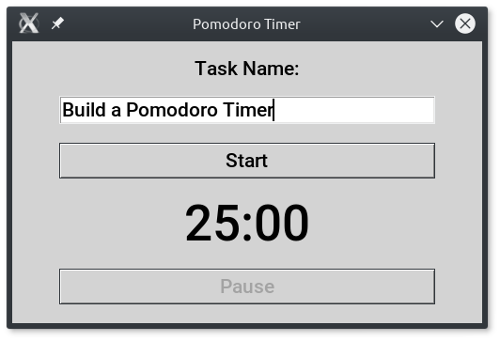
\includegraphics{Ch7-1}
\caption{A Pomodoro Timer}
\end{figure}

\lstinputlisting[language=Python, caption=A 25 Minute Timer, captionpos=b]{Code/Chapter7-1.py}

\subsection{Timer}

\subsubsection{\_\_init\_\_}

Everything in \lstinline[columns=fixed]{__init__} should look familiar now. We create a \lstinline[columns=fixed]{Frame} which holds all of our content. We have a \lstinline[columns=fixed]{Label} which tells the user what to put in the \lstinline[columns=fixed]{Entry}, a start \lstinline[columns=fixed]{Button}, another \lstinline[columns=fixed]{Label} holding the time remaining, and a pause \lstinline[columns=fixed]{Button}. Within the pomodoro technique tasks aren't actually supposed to be paused, but life happens, so it may come in handy. Note that the pause \lstinline[columns=fixed]{Button} is disabled by default, since we cannot pause a timer until it has begun. 

\vspace{5mm}

We pack everything to fill the x direction giving us a single column layout. We use some padding to separate widgets vertically and to pull them off of the sides of the window. We then bind a method - \lstinline[columns=fixed]{safe_destroy} - to the window close. This will be explained later. 

\subsubsection{setup\_worker}

Our "worker" is going to be a separate thread which will hold a reference to our \lstinline[columns=fixed]{Timer} instance and call functions on it to update its widgets. Since a thread can only be run once, we cannot just set this up in our \lstinline[columns=fixed]{__init__} and then call \lstinline[columns=fixed]{run} each time we want to start a timer, we instead need to create a new instance each time. That's why we have this separate method. 

\vspace{5mm}

To set up our \lstinline[columns=fixed]{CountingThread} we need to give it a \lstinline[columns=fixed]{start_time} and an \lstinline[columns=fixed]{end_time}. As this method will only be run upon starting the timer, we can use \lstinline[columns=fixed]{datetime.datetime.now()} to get the current time as our \lstinline[columns=fixed]{start_time}. Since the pomodoro technique works in 25 minute blocks, we create our \lstinline[columns=fixed]{end_time} by adding on a \lstinline[columns=fixed]{datetime.timedelta(minutes=25)}. We create our \lstinline[columns=fixed]{CountingThread} with these arguments and assign it to our \lstinline[columns=fixed]{Timer} as \lstinline[columns=fixed]{self.worker}.  

\subsubsection{start}

If we don't have a worker, we will set one up. We then disable our \lstinline[columns=fixed]{task_name_entry} and enable our \lstinline[columns=fixed]{pause_button}, swap our \lstinline[columns=fixed]{start_button} to a finish button, set the time \lstinline[columns=fixed]{Label} to "25:00", and finally start off our worker. 

\subsubsection{pause}

We use \lstinline[columns=fixed]{not} to flip the paused attribute of our worker, allowing this function to work as both a pause and resume. If the worker is now paused we change the pause button to say "Resume" and set the current time as our worker's \lstinline[columns=fixed]{start_time}. This will allow us to keep track of how long we were paused for an adjust the \lstinline[columns=fixed]{end_time} accordingly.

\vspace{5mm}

On unpausing we set the button text back to "Pause" and calculate how long we were paused for by subtracting the \lstinline[columns=fixed]{start_time} from the current time. This amount now needs to be added on to the worker's \lstinline[columns=fixed]{end_time} to account for the time paused. 

\subsubsection{finish}

Upon finishing we revert things back to their initial state, enabling our \lstinline[columns=fixed]{task_name_entry}, disabling our \lstinline[columns=fixed]{pause_button}, setting our clock back to "25:00", and changing our finish button back to a start button. We delete the reference to our worker as we no longer need it, since threads can only run once, before alerting the user that their time is up.

\subsubsection{finish\_early}
If finishing early (by clicking the finish button which replaced our start button) We just need to swap the finish button back to a start button and set the \lstinline[columns=fixed]{end_now} variable of our worker to \lstinline[columns=fixed]{True}, which will set it up to handle the rest. 

\subsubsection{update\_time\_remaining}
To update the timer on screen we simply call \lstinline[columns=fixed]{set} on our \lstinline[columns=fixed]{time_remaining_var} with the time returned from our \lstinline[columns=fixed]{CountingThread}. We then call \lstinline[columns=fixed]{update_idletasks} which forces the app to refresh its display. Without this the timer may occasionally appear to miss seconds. 

\subsubsection{safe\_destroy}
If the user was to start the timer and then close the window they would be left with a running thread still. In this case it seems as if the thread will throw an exception when it cannot reach the \lstinline[columns=fixed]{Timer} instance and exit, but it is always best to ensure you do not leave an application with active threads still remaining. This ties up system resources and makes the user have to close them via some sort of task manager. 

\vspace{5mm}

In our \lstinline[columns=fixed]{safe_destroy} method we check to see if we have an assigned worker. If so this means the user has started the timer. We set the \lstinline[columns=fixed]{force_quit} attribute of our worker to \lstinline[columns=fixed]{True} which will cause it to \lstinline[columns=fixed]{return} out of its \lstinline[columns=fixed]{run} method and complete its duty. Before doing so it will \lstinline[columns=fixed]{del} the reference in our \lstinline[columns=fixed]{Timer} instance so that we know it has successfully ended. We use \lstinline[columns=fixed]{self.after} to call this same method again every 100 milliseconds until the worker has removed the reference to itself from our \lstinline[columns=fixed]{Timer}, in which case we are free to \lstinline[columns=fixed]{destroy} the \lstinline[columns=fixed]{Timer}. 

\vspace{5mm}

Now let's have a look at exactly how our \lstinline[columns=fixed]{CountingThread} works:

\subsection{CountingThread}

\subsubsection{\_\_init\_\_ and run}

Hopefully \lstinline[columns=fixed]{__init__} is self explanitory, we are just setting up some variables. \lstinline[columns=fixed]{master} will be our main window, \lstinline[columns=fixed]{start_time} and \lstinline[columns=fixed]{end_time} will be timestamps of when the pomodoro should start and end, and then we have 3 variables which keep track of whether or not the thread should continue running its loop. 

\vspace{5mm}

\lstinline[columns=fixed]{run} contains an infinite loop which first checks that none of our three variables which indicate that the loop should stop are true. If they aren't it will run its main loop to do some calculations and update the GUI. If the current time is past the set \lstinline[columns=fixed]{end_time} we will signal to the \lstinline[columns=fixed]{Timer} to \lstinline[columns=fixed]{finish}. 

\vspace{5mm}

If \lstinline[columns=fixed]{end_now} is set, this means the user is finishing the task early, so this will jump to the finish method too. If \lstinline[columns=fixed]{force_quit} is set then the user has closed the application window whilst the thread is still running, so we need to remove the thread from the main \lstinline[columns=fixed]{Timer} before returning, which will end the thread. 

\vspace{5mm}

The final \lstinline[columns=fixed]{else continue} is hit when the \lstinline[columns=fixed]{Timer} is paused, so the \lstinline[columns=fixed]{CountingThread} needs to do nothing but still remain in its loop. 

\subsubsection{main\_loop}

In this method we need to find out the amount of time remaining and update the \lstinline[columns=fixed]{Timer}'s clock appropriately. We grab the current time with \lstinline[columns=fixed]{datetime.datetime.now()} and check if it's still less than our \lstinline[columns=fixed]{end_time}. If it is we calculate the difference. We then use \lstinline[columns=fixed]{divmod} to get the time in minutes and seconds which we can use with \lstinline[columns=fixed]{.format} to create our next time string. We check once again for \lstinline[columns=fixed]{force_quit} just to be sure before passing the time to \lstinline[columns=fixed]{update_time_remaining}.  

\subsection{Next Iteration}

Now that we have a basic timer application working we can build up some useful features to go along with it. Next iteration we will add a log screen to display finished tasks which have been stored in a sqlite database. 

\newpage

\section{Keeping a Log}

\lstinputlisting[language=Python, caption=A Timer With a Log, captionpos=b]{Code/Chapter7-2-abridged.py}

\subsection{Timer}

There should be some nostalgia when working through this chapter, as a lot of code has been taken from Chapter 2. Most notably: \lstinline[columns=fixed]{runQuery} and \lstinline[columns=fixed]{firstTimeDb}. 

\vspace{5mm}

When setting up our \lstinline[columns=fixed]{Timer} instance we now have a \lstinline[columns=fixed]{Menu} with a button to open the log. This is also bound to Control-L. 

\vspace{5mm}

Upon starting a task, if there's no task name in our \lstinline[columns=fixed]{task_name_entry} we will inform the user with a messagebox. You may have noticed that the \lstinline[columns=fixed]{task_name_entry} was kind of pointless in the previous iteration, but now we have a database connected we will need the ability to name each task. We also have a boolean \lstinline[columns=fixed]{task_finished_early} which will be used to mark whether or not a task was executed for the full 25 minutes. Within our \lstinline[columns=fixed]{finish_early} method we will set this to \lstinline[columns=fixed]{True} which affects whether or not the record is updated when we get to \lstinline[columns=fixed]{finish}. 

\vspace{5mm}

When we first \lstinline[columns=fixed]{start} a task we add an entry into the database with the task's name and the date/time it started (via \lstinline[columns=fixed]{add_new_task}). It is initially marked as not being worked on for the full 25 minutes. Once we hit the \lstinline[columns=fixed]{finish} method we will update the value of the \lstinline[columns=fixed]{finished} column if the task was not finished early (with \lstinline[columns=fixed]{mark_finished_task}).

\vspace{5mm}

When creating and running our \lstinline[columns=fixed]{Timer} instance, we will call \lstinline[columns=fixed]{firstTimeDb} if the database file does not exist in the same directory as the app. This is the same as we did in Chapter 2 for our Todo list. 

\subsection{LogWindow}

The \lstinline[columns=fixed]{LogWindow} consists of two widgets from the ttk set: a \lstinline[columns=fixed]{Notebook}, which we met in Chapter 3, and a \lstinline[columns=fixed]{Treeview}. The \lstinline[columns=fixed]{Notebook} is used to create a tabbed interface inside the window, and the \lstinline[columns=fixed]{Treeview} will organise our information into a neat little table. This saves us from having to manually lay the information out using \lstinline[columns=fixed]{Label}s.

\vspace{5mm}

We query our database for a list of dates then \lstinline[columns=fixed]{enumerate} over them to replace each full \lstinline[columns=fixed]{datetime} with just the date part. We need to use \lstinline[columns=fixed]{date[0]} for each record as sqlite returns even single items in a \lstinline[columns=fixed]{tuple}. We then use the somewhat strange looking \lstinline[columns=fixed]{dates = sorted(set(dates), reverse=True)} to get a list of unique dates in descending order. We first cast the \lstinline[columns=fixed]{list} to a \lstinline[columns=fixed]{set} in order to remove duplicates, then \lstinline[columns=fixed]{sorted} with \lstinline[columns=fixed]{reverse=True} to order them descending. That way today's items are always first. 

\vspace{5mm}

We once again loop over our now-ordered dates and create a new \lstinline[columns=fixed]{Frame}, which will function as a tab in our \lstinline[columns=fixed]{Notebook}, for each date. The tuple of strings will function as identifiers for each column and the \lstinline[columns=fixed]{show="headings"} removes the default "icon" column from the \lstinline[columns=fixed]{Treeview}. Without this we would get a blank first column. We use three calls to \lstinline[columns=fixed]{.heading} to configure each column's heading, followed by three calls to \lstinline[columns=fixed]{.column} to center-align our data. 

\vspace{5mm}

Another query is run against our database to get all of the tasks which match the current date. We iterate over the results formatting the data in a friendlier way, and getting the times rather than the dates (since the date is written on the tab) before using \lstinline[columns=fixed]{insert} to add the information into our \lstinline[columns=fixed]{Treeview}. The blank string as the first argument tells the \lstinline[columns=fixed]{Treeview} that this record has no parent, and the \lstinline[columns=fixed]{tk.END} tells it to insert each record after all others. We then \lstinline[columns=fixed]{pack} our \lstinline[columns=fixed]{Treeview} into the tab and add the tab to our \lstinline[columns=fixed]{Notebook}. 

\vspace{5mm}

Once this has been done for each date, we finish off by \lstinline[columns=fixed]{pack}ing our \lstinline[columns=fixed]{Notebook}. With that our \lstinline[columns=fixed]{LogWindow} is complete. Give it a go by running a couple of tasks then pressing Control-L to pop open the log. 

\begin{figure}[h]
\centering
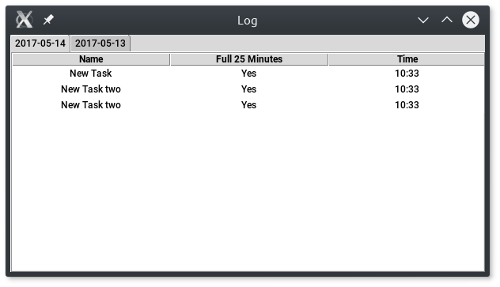
\includegraphics{Ch7-2}
\caption{Our Log Window}
\end{figure}

\subsection{Next Iteration}

We'll finish up our timer by styling the \lstinline[columns=fixed]{Treeview} using ttk's \lstinline[columns=fixed]{Style} objects, as well as neatening up the main window by replacing some tk widgets with the ttk equivalent. We'll also add delete functionality via the log. 

\newpage

\section{Our Finished Timer}

\lstinputlisting[language=Python, caption=Our ttk Timer, captionpos=b]{Code/Chapter7-3-abridged.py}

\subsection{Timer}

\subsubsection{\_\_init\_\_}

Our widgets have now been swapped to their ttk counterparts and the styling options have been removed from their creation arguments. Ttk aims to keep declaration of widgets separate from their styling, meaning they will no longer support keyword arguments like \lstinline[columns=fixed]{bg} when creating the instances. We instead create and use a \lstinline[columns=fixed]{ttk.Style} object in order to adjust how our widgets look.

\vspace{5mm}

To achieve this we create a \lstinline[columns=fixed]{Style} object and use its \lstinline[columns=fixed]{configure} method to adjust style elements. Each ttk widget will have an associated class with which it gathers styling - usually a capital T followed by the object name, such as \lstinline[columns=fixed]{TButton} or \lstinline[columns=fixed]{TLabel} - but there are a couple of exceptions. The first argument to the \lstinline[columns=fixed]{configure} method is the name of the style class we are changing and the following keyword arguments signify what we are changing. 

\vspace{5mm}

When we configure \lstinline[columns=fixed]{TLabel} in the first instance we are changing \textit{all} \lstinline[columns=fixed]{Label}s throughout our application. This is fine for us here as we only have two which both want the same colouring. We cannot do this for the \lstinline[columns=fixed]{Button} class however as this affects the \lstinline[columns=fixed]{Button}s which appear in \lstinline[columns=fixed]{messagebox}es. 

\vspace{5mm}

In order to "subclass" a style we use a kind of dot-notation to specify inheritance. In our code you will see we define \lstinline[columns=fixed]{B.TLabel}. This style inherits from the global \lstinline[columns=fixed]{TLabel} we adjusted and allows us to build on top of it. In this case we want to inherit the colouring but increase the font size (the B stands for Big). Styling in this way prevents us from having to type \lstinline[columns=fixed]{bg="lightgrey", fg="black"} for each widget. 

\vspace{5mm}

We go on to define a Big \lstinline[columns=fixed]{Button} styling with \lstinline[columns=fixed]{B.TButton} and some global \lstinline[columns=fixed]{Entry} styling with \lstinline[columns=fixed]{TEntry}. Note that the font of an \lstinline[columns=fixed]{Entry} cannot be set with the styling, so must be set upon creation as before. 

\vspace{5mm}

To apply the non-global styles to our widgets we use the \lstinline[columns=fixed]{style} keyword. Each one will default to the global (\lstinline[columns=fixed]{TButton, TLabel,} etc) and if we want to specify an inherited style we pass the full style class as the argument. You can see this being done with our \lstinline[columns=fixed]{Button}s using "B.TButton" and our \lstinline[columns=fixed]{time_remaining_label} using "B.TLabel". 

\vspace{5mm}

We finish up our changes to \lstinline[columns=fixed]{__init__} by setting focus to the \lstinline[columns=fixed]{task_name_entry} when the user opens the app so that they don't have to click into it to begin typing. 

\subsubsection{Managing Tasks}

All of the SQL has been moved from the \lstinline[columns=fixed]{LogWindow} into the \lstinline[columns=fixed]{Timer} for consistency. The two queries which should look familiar are \lstinline[columns=fixed]{get_unique_dates} and \lstinline[columns=fixed]{get_tasks_by_date}. 

\vspace{5mm}

\lstinline[columns=fixed]{delete_task} handles removing a task when it is double-clicked in the \lstinline[columns=fixed]{LogWindow} (we will get to that soon). 

\vspace{5mm}

\lstinline[columns=fixed]{task_is_duplicate} is used to check whether we have a task with the same name on the current date. This is because we don't have a unique identifier for each task and we want to make sure we only delete one task at a time. If we had three tasks called "test" all done at the same time we would end up deleting them all when double clicking one of them in the log. We call this method from our \lstinline[columns=fixed]{start} method and show a \lstinline[columns=fixed]{messagebox} with an error if a task already exists.  


\subsection{LogWindow} 

\subsubsection{Styling}
The \lstinline[columns=fixed]{Treeview} widget is one of the exceptions mentioned earlier when it comes to naming ttk \lstinline[columns=fixed]{Style}s. Its class is just "Treeview" not "TTreeview". We use the \lstinline[columns=fixed]{Style} to configure the font size of the items within our table. In order to change the font used in the headings we need to adjust the \lstinline[columns=fixed]{Treeview.Heading} class. Again both of these \lstinline[columns=fixed]{configure}s apply globally to all \lstinline[columns=fixed]{Treeview}s in our app. 

\subsubsection{Deleting}

In order to get our delete functinality to work we need to bind double-click (\lstinline[columns=fixed]{<Double-Button-1>} in tkinter) events to each \lstinline[columns=fixed]{Treeview}. We also need to keep track of what \lstinline[columns=fixed]{Treeview}s we have and which date they belong to. We do this using a dictionary called \lstinline[columns=fixed]{tab_trees}. The key is the date and the item is the \lstinline[columns=fixed]{Treeview} itself. Since our \lstinline[columns=fixed]{Notebook} tabs are named after the dates this will allow us to access the relevant \lstinline[columns=fixed]{Treeview} for the current tab. 

\vspace{5mm}

Within \lstinline[columns=fixed]{confirm_delete} we use the \lstinline[columns=fixed]{tab} method of our \lstinline[columns=fixed]{Notebook} to get the "text" attribute from our currently selected tab. This gives us the date of the tab currently being looked at. We use this date to fish out the relevant \lstinline[columns=fixed]{Treeview} from \lstinline[columns=fixed]{tab_trees} and grab the selected item's ID with \lstinline[columns=fixed]{selection()}. We pass this ID to the \lstinline[columns=fixed]{item} method in order to get a dictionary containing its information. If you want to see this dictionary add \lstinline[columns=fixed]{print(selected_item)} after this line. The values of this item are stored within the "values" section of the dictionary. 

\vspace{5mm}

We use an \lstinline[columns=fixed]{askyesno messagebox} to confirm whether the user wants to delete this record. If so we get the task name and time from the "values", merge the date with the task time for specificity with delete statement, and then pass this information over to \lstinline[columns=fixed]{delete_task} in our \lstinline[columns=fixed]{Timer}. We finish off by calling the \lstinline[columns=fixed]{delete} method of our tree to remove the item from the screen without having to re-build the whole page. 

\vspace{5mm}

That's where we'll leave our pomodoro timer. We now have a 25 minute timer which contains a full log of all of our tasks, all handled automatically. We can also remove any tasks which we didn't want logged for any reason.

\subsection{Further Development}

If you'd like to continue work on this project as an exercise, try the following:

\begin{itemize}
  \item Add scrolling to our log for those days when we are super productive.
  \item Add a way to re-order the tabs to be either ascending or descending.
  \item Add a to-do list to the app and have a way to select an item and have it auto-populate the task name entry.
  \item Allow the user to vary the timer length. 
\end{itemize} 

\chapter{Miscellaneous}

That's it for all of the projects within this book. I hope you've learned enough to start developing your own GUI application with tkinter. I haven't covered absolutely everything in this book since I wanted all of the examples to be real, useful applications as opposed to small demonstrations of widgets. In this final chapter we'll just have a brief look at some things which I think will be useful to know but I didn't manage to cover in my examples. 

\section{Alternate Geometry Managers}

\subsection{Grid}

Grid is a geometry manager with the same job as pack: to place your widgets into their parent. As you may have guessed from the name, \lstinline[columns=fixed]{grid} treats your window as a literal grid and allows you to place widgets into a "cell" at a certain \lstinline[columns=fixed]{row} and \lstinline[columns=fixed]{column}. Their horizontal size is handled with \lstinline[columns=fixed]{colspan} and the vertical size with \lstinline[columns=fixed]{rowspan}. Widgets will expand via the use of a \lstinline[columns=fixed]{sticky} argument which takes a combination of "n", "s", "e", and "w" (north, south, east, west). This will make it stick to the particular end of its cell, so a \lstinline[columns=fixed]{sticky} of "we" means the widget will stretch horizontally within its assigned cell. Widgets default to the center of their cell if there is no \lstinline[columns=fixed]{sticky} value set. 

\vspace{5mm}

We can \lstinline[columns=fixed]{grid} widgets in any order we like, providing we specify their values correctly, since each one is assigned to a specific cell (or group of cells). With \lstinline[columns=fixed]{pack} the order in which we \lstinline[columns=fixed]{pack} our widgets defines their position. For example, when we are \lstinline[columns=fixed]{packing} two \lstinline[columns=fixed]{Buttons} with \lstinline[columns=fixed]{side=tk.BOTTOM}, the first Button which is \lstinline[columns=fixed]{pack}ed will appear at the very bottom, with the second above it. When adding more \lstinline[columns=fixed]{Button}s to the bottom of this window, we must ensure we \lstinline[columns=fixed]{pack} them after the first one if we want to keep it at the bottom, whereas with \lstinline[columns=fixed]{grid} we can just specify a smaller \lstinline[columns=fixed]{row} value, and then \lstinline[columns=fixed]{grid} it whenever we like. 

\vspace{5mm}

The other main advantage of \lstinline[columns=fixed]{grid} is that we don't have to use \lstinline[columns=fixed]{Frame}s if we wish to specify two \lstinline[columns=fixed]{side}s. For example, take our find window from the text editor in chapter 6. In order to place our \lstinline[columns=fixed]{Button}s both at the bottom of the window and side-by-side we had to use a \lstinline[columns=fixed]{Frame pack}ed to the bottom, then \lstinline[columns=fixed]{pack} each widget to the left. If using \lstinline[columns=fixed]{grid} we wouldn't need the extra \lstinline[columns=fixed]{Frame}, we could simply give all of the \lstinline[columns=fixed]{Button}s the same \lstinline[columns=fixed]{row}. 
 
\vspace{5mm}

The reason I don't tend to use grid is simply because I find it unflexible when developing iteratively. If we accidentally \lstinline[columns=fixed]{grid} a widget in the same \lstinline[columns=fixed]{row} and \lstinline[columns=fixed]{column} as another it will just overtake that cell, hiding the first widget. This means each time we want to add something we would potentially have to adjust the \lstinline[columns=fixed]{row} and \lstinline[columns=fixed]{column} of multiple other widgets. 

\vspace{5mm}

I also find \lstinline[columns=fixed]{pack} to be typically more readable than \lstinline[columns=fixed]{grid}. Instead of having to compare numbers across multiple widgets to get a mental picture of what goes where, we have words like "bottom" and "left" right there in the code. 

\vspace{5mm}

Despite my opinions, \lstinline[columns=fixed]{grid} is a powerful tool, so if you feel it is better for the job than \lstinline[columns=fixed]{pack} then I encourage you to use it. For some great examples with pictures check out the tkinterbook page over at \lstinline[columns=fixed]{effbot.org/tkinterbook/grid.htm}. 

\subsection{Place}

If you want to specify exact coordinates within the window to put something, \lstinline[columns=fixed]{place} will do that for you. It's generally a pain to lay a window out with specifics, and there's much less room for the widgets to adapt with the window size, so \lstinline[columns=fixed]{place} sees very little use. 

\vspace{5mm}

To put a widget at (100, 300) within a window, use \lstinline[columns=fixed]{widget.place(x=100, y=500)}. Alternatively, you can use \lstinline[columns=fixed]{relx} and \lstinline[columns=fixed]{rely} to \lstinline[columns=fixed]{place} a widget relative to its parent. \lstinline[columns=fixed]{relx=0.5, rely=0.5, anchor=tk.CENTER} will keep a widget completely central in its parent. 

\vspace{5mm}

\lstinline[columns=fixed]{place}d widgets will overlap anything underneath them. This can be good or bad depending on your intentions.

\section{Tk Widgets}

There are still some widgets which I didn't manage to fit into any of the example apps. We'll have a brief overview of them here:

\subsection{Checkbutton}

A \lstinline[columns=fixed]{Checkbutton} is essentially a checkbox with an attached label. The label is set with the \lstinline[columns=fixed]{text} argument much like the other \lstinline[columns=fixed]{tkinter} widgets. We can query whether or not the box has been checked by attaching a \lstinline[columns=fixed]{tkinter} variable to it (\lstinline[columns=fixed]{StringVar, IntVar} etc) with \lstinline[columns=fixed]{variable=self.my_variable}. By deault the value of this variable will be 1 when checked and 0 when not. We can change this with the \lstinline[columns=fixed]{onvalue} and \lstinline[columns=fixed]{offvalue} arguments. Changing the linked variable directly will update the associated \lstinline[columns=fixed]{Checkbutton} automatically. 

\vspace{5mm}

Much like a normal \lstinline[columns=fixed]{Button}, a \lstinline[columns=fixed]{Checkbutton} can take a \lstinline[columns=fixed]{command} argument to call a function whenever it is pressed.

\subsection{Radiobutton} 

Somewhat similar to a \lstinline[columns=fixed]{Checkbutton}, a \lstinline[columns=fixed]{Radiobutton} is used to represent one choice out of a group of possible options. To group \lstinline[columns=fixed]{Radiobutton}s, point them all to the same \lstinline[columns=fixed]{tkinter} variable using the \lstinline[columns=fixed]{variable} keyword. Each \lstinline[columns=fixed]{Radiobutton} can then have its own unique value assigned with the \lstinline[columns=fixed]{value} keyword, which becomes the value of the linked variable when this \lstinline[columns=fixed]{Radiobutton} is selected. 

\vspace{5mm}

Once again, the \lstinline[columns=fixed]{text} argument will put a label beside the button. We can also bind a function via \lstinline[columns=fixed]{command}.

\vspace{5mm}

By default a \lstinline[columns=fixed]{Radiobutton} will look like it does on a standard HTML page (circular icon next to text with a dot inside the selected option). If you wish instead to have each option look like a regular button with the chosen option pressed in, setting the \lstinline[columns=fixed]{indicatoron} argument to false will do this. 

\subsection{Checkbuttons and Radiobuttons in a Menu}

A \lstinline[columns=fixed]{Menu} can take contain \lstinline[columns=fixed]{Checkbutton}s and \lstinline[columns=fixed]{Radiobuttons} as well as the normal \lstinline[columns=fixed]{Button}s we used in our projects. These are added with \lstinline[columns=fixed]{.add_checkbutton(label="check", variable=self.checked)} and \lstinline[columns=fixed]{.add_radiobutton(label="radio", variable=self.radio)}. The buttons will be linked to the supplied \lstinline[columns=fixed]{tkinter} variable just like regular \lstinline[columns=fixed]{Checkbutton}s and \lstinline[columns=fixed]{Radiobutton}s.

\subsection{OptionMenu}

An \lstinline[columns=fixed]{OptionMenu} is much like an HTML dropdown box. Unlike other \lstinline[columns=fixed]{tkinter} widgets the \lstinline[columns=fixed]{OptionMenu} doesn't rely on keyword arguments when creating an instance. Instead, instances are created like this: \lstinline[columns=fixed]{om = OptionMenu(parent, variable, "option1", "option2", "option3")}. In this case \lstinline[columns=fixed]{parent} is your root window, \lstinline[columns=fixed]{variable} is a \lstinline[columns=fixed]{tkinter} variable, and all of the following arguments are the options to choose from in the box. 

\vspace{5mm}

If developing for Windows or OSX I would recommend using the \lstinline[columns=fixed]{ttk} version of \lstinline[columns=fixed]{OptionMenu} (and any ttk-supported widget to be honest), since it looks so much nicer. One thing to note with this version is the third argument will become the default. To clarify, we create an instance with \lstinline[columns=fixed]{OptionMenu(parent, variable, "default choice", "choice 1", "choice2")}. The default choice will \textit{not} appear in the list of available options unless re-declared as the 4th or higher argument, eg \lstinline[columns=fixed]{(parent, variable, "medium", "low", "medium", "high")}.

\vspace{5mm}

A nicer way to specify the potential choices is to create a \lstinline[columns=fixed]{tuple} and then unpack it when creating the \lstinline[columns=fixed]{OptionMenu}, eg \lstinline[columns=fixed]{(parent, variable, *choices)}.

\section{Ttk Widgets}

\subsection{Combobox}

A \lstinline[columns=fixed]{Combobox} is a combination of an \lstinline[columns=fixed]{Entry} and an \lstinline[columns=fixed]{OptionMenu}. The user can either pick an option from the dropdown list or type their own. This is sometimes called a "select2" in the web development world. Unfortunately, typing in the \lstinline[columns=fixed]{Entry} does not filter the values in the dropdown by default, so if that is your intention you will need to implement this manually. This can either be done by binding to the \lstinline[columns=fixed]{<KeyRelease>} event, or by using the \lstinline[columns=fixed]{postcommand} argument to bind a function which will run when the user clicks the dropdown arrow. 

\vspace{5mm}

A \lstinline[columns=fixed]{Combobox} can be instantiated by passing the parent as the first argument followed by the values as a sequence of strings. For example: \lstinline[columns=fixed]{Combobox(parent, values=("one", "two", "three"))}. This widget can also be bound to a \lstinline[columns=fixed]{StringVar} with the \lstinline[columns=fixed]{textvariable} argument. 

\subsection{Progressbar}

When running something which may take a long time we can use a \lstinline[columns=fixed]{Progressbar} to let the user know that the application has not crashed. 

\vspace{5mm}

If you have a quantifiable end goal, such as a number of open files to process, you can use a \lstinline[columns=fixed]{determinate Progressbar} to show exactly how far through the process your application currently is. Determinate is the default mode of the \lstinline[columns=fixed]{Progressbar} widget. Let's say you had a big list of open files to process - you would show the progress like so: \lstinline[columns=fixed]{pb = Progressbar(parent, maximum=len(files))}. You now have a \lstinline[columns=fixed]{Progressbar} with step count equal to the length of your file list. After processing each file, you can call \lstinline[columns=fixed]{pb.step()} to increment progress by one. Once the \lstinline[columns=fixed]{Progressbar} has reached its \lstinline[columns=fixed]{maximum} it will return to empty, so you should \lstinline[columns=fixed]{destroy} it (or its parent if it has a separate window).

\vspace{5mm}

If you have no idea how much work there is to do but still want to signal to the user that the app is processing, there is the \lstinline[columns=fixed]{mode="indeterminate"} argument. This will create one of those animations where a small block bounces left and right until processing is complete. To begin this animation call \lstinline[columns=fixed]{pb.start()}, and use \lstinline[columns=fixed]{pb.stop()} when processing is complete (or use \lstinline[columns=fixed]{destroy()} as before). 

\vspace{5mm}

The length of a \lstinline[columns=fixed]{Progressbar} can be set with the \lstinline[columns=fixed]{length} argument, and for some reason you can also set it to vertical with \lstinline[columns=fixed]{orient=tk.VERTICAL}.

\section{Final Words}

With that, we have come to the end of this book. Thanks very much for reading. I would love to hear your thoughts on this book - you can find me @Dvlv292 on twitter or Dvlv on reddit. Any comments, questions, or suggestions on the source code can be handled through Github. I am more than happy to alter the code and this book in order to improve it for people new to tkinter. As always in programming - nothing is ever finished! 





\end{document}
